\documentclass[twoside]{book}

% Packages required by doxygen
\usepackage{fixltx2e}
\usepackage{calc}
\usepackage{doxygen}
\usepackage[export]{adjustbox} % also loads graphicx
\usepackage{graphicx}
\usepackage[utf8]{inputenc}
\usepackage{makeidx}
\usepackage{multicol}
\usepackage{multirow}
\PassOptionsToPackage{warn}{textcomp}
\usepackage{textcomp}
\usepackage[nointegrals]{wasysym}
\usepackage[table]{xcolor}

% Font selection
\usepackage[T1]{fontenc}
\usepackage[scaled=.90]{helvet}
\usepackage{courier}
\usepackage{amssymb}
\usepackage{sectsty}
\renewcommand{\familydefault}{\sfdefault}
\allsectionsfont{%
  \fontseries{bc}\selectfont%
  \color{darkgray}%
}
\renewcommand{\DoxyLabelFont}{%
  \fontseries{bc}\selectfont%
  \color{darkgray}%
}
\newcommand{\+}{\discretionary{\mbox{\scriptsize$\hookleftarrow$}}{}{}}

% Page & text layout
\usepackage{geometry}
\geometry{%
  a4paper,%
  top=2.5cm,%
  bottom=2.5cm,%
  left=2.5cm,%
  right=2.5cm%
}
\tolerance=750
\hfuzz=15pt
\hbadness=750
\setlength{\emergencystretch}{15pt}
\setlength{\parindent}{0cm}
\setlength{\parskip}{3ex plus 2ex minus 2ex}
\makeatletter
\renewcommand{\paragraph}{%
  \@startsection{paragraph}{4}{0ex}{-1.0ex}{1.0ex}{%
    \normalfont\normalsize\bfseries\SS@parafont%
  }%
}
\renewcommand{\subparagraph}{%
  \@startsection{subparagraph}{5}{0ex}{-1.0ex}{1.0ex}{%
    \normalfont\normalsize\bfseries\SS@subparafont%
  }%
}
\makeatother

% Headers & footers
\usepackage{fancyhdr}
\pagestyle{fancyplain}
\fancyhead[LE]{\fancyplain{}{\bfseries\thepage}}
\fancyhead[CE]{\fancyplain{}{}}
\fancyhead[RE]{\fancyplain{}{\bfseries\leftmark}}
\fancyhead[LO]{\fancyplain{}{\bfseries\rightmark}}
\fancyhead[CO]{\fancyplain{}{}}
\fancyhead[RO]{\fancyplain{}{\bfseries\thepage}}
\fancyfoot[LE]{\fancyplain{}{}}
\fancyfoot[CE]{\fancyplain{}{}}
\fancyfoot[RE]{\fancyplain{}{\bfseries\scriptsize Generated by Doxygen }}
\fancyfoot[LO]{\fancyplain{}{\bfseries\scriptsize Generated by Doxygen }}
\fancyfoot[CO]{\fancyplain{}{}}
\fancyfoot[RO]{\fancyplain{}{}}
\renewcommand{\footrulewidth}{0.4pt}
\renewcommand{\chaptermark}[1]{%
  \markboth{#1}{}%
}
\renewcommand{\sectionmark}[1]{%
  \markright{\thesection\ #1}%
}

% Indices & bibliography
\usepackage{natbib}
\usepackage[titles]{tocloft}
\setcounter{tocdepth}{3}
\setcounter{secnumdepth}{5}
\makeindex

% Hyperlinks (required, but should be loaded last)
\usepackage{ifpdf}
\ifpdf
  \usepackage[pdftex,pagebackref=true]{hyperref}
\else
  \usepackage[ps2pdf,pagebackref=true]{hyperref}
\fi
\hypersetup{%
  colorlinks=true,%
  linkcolor=blue,%
  citecolor=blue,%
  unicode%
}

% Custom commands
\newcommand{\clearemptydoublepage}{%
  \newpage{\pagestyle{empty}\cleardoublepage}%
}

\usepackage{caption}
\captionsetup{labelsep=space,justification=centering,font={bf},singlelinecheck=off,skip=4pt,position=top}

%===== C O N T E N T S =====

\begin{document}

% Titlepage & ToC
\hypersetup{pageanchor=false,
             bookmarksnumbered=true,
             pdfencoding=unicode
            }
\pagenumbering{roman}
\begin{titlepage}
\vspace*{7cm}
\begin{center}%
{\Large V\+R\+E\+P-\/\+Plugin for paparazzi communication to control simulated copters }\\
\vspace*{1cm}
{\large Generated by Doxygen 1.8.11}\\
\end{center}
\end{titlepage}
\clearemptydoublepage
\tableofcontents
\clearemptydoublepage
\pagenumbering{arabic}
\hypersetup{pageanchor=true}

%--- Begin generated contents ---
\chapter{Hierarchical Index}
\section{Class Hierarchy}
This inheritance list is sorted roughly, but not completely, alphabetically\+:\begin{DoxyCompactList}
\item \contentsline{section}{Async\+\_\+\+Server}{\pageref{classAsync__Server}}{}
\item \contentsline{section}{ecef\+\_\+coords}{\pageref{structecef__coords}}{}
\item \contentsline{section}{Finken}{\pageref{classFinken}}{}
\item \contentsline{section}{finken\+P\+ID}{\pageref{classfinkenPID}}{}
\item \contentsline{section}{lla\+\_\+coords}{\pageref{structlla__coords}}{}
\item \contentsline{section}{Log}{\pageref{classLog}}{}
\item \contentsline{section}{Log\+Line}{\pageref{classLogLine}}{}
\item \contentsline{section}{Rotor}{\pageref{classRotor}}{}
\item \contentsline{section}{Sensor}{\pageref{classSensor}}{}
\begin{DoxyCompactList}
\item \contentsline{section}{Attitude\+Sensor}{\pageref{classAttitudeSensor}}{}
\item \contentsline{section}{Height\+Sensor}{\pageref{classHeightSensor}}{}
\item \contentsline{section}{Position\+Sensor}{\pageref{classPositionSensor}}{}
\item \contentsline{section}{Sonar}{\pageref{classSonar}}{}
\end{DoxyCompactList}
\item \contentsline{section}{Sync}{\pageref{structSync}}{}
\item \contentsline{section}{Vrep\+Log}{\pageref{classVrepLog}}{}
\item \contentsline{section}{V\+R\+E\+P\+Plugin}{\pageref{classVREPPlugin}}{}
\begin{DoxyCompactList}
\item \contentsline{section}{Finken\+Plugin}{\pageref{classFinkenPlugin}}{}
\end{DoxyCompactList}
\end{DoxyCompactList}

\chapter{Class Index}
\section{Class List}
Here are the classes, structs, unions and interfaces with brief descriptions\+:\begin{DoxyCompactList}
\item\contentsline{section}{\hyperlink{classAsync__Server}{Async\+\_\+\+Server} }{\pageref{classAsync__Server}}{}
\item\contentsline{section}{\hyperlink{classAttitudeSensor}{Attitude\+Sensor} }{\pageref{classAttitudeSensor}}{}
\item\contentsline{section}{\hyperlink{structecef__coords}{ecef\+\_\+coords} }{\pageref{structecef__coords}}{}
\item\contentsline{section}{\hyperlink{classFinken}{Finken} }{\pageref{classFinken}}{}
\item\contentsline{section}{\hyperlink{classfinkenPID}{finken\+P\+ID} }{\pageref{classfinkenPID}}{}
\item\contentsline{section}{\hyperlink{classFinkenPlugin}{Finken\+Plugin} }{\pageref{classFinkenPlugin}}{}
\item\contentsline{section}{\hyperlink{classHeightSensor}{Height\+Sensor} }{\pageref{classHeightSensor}}{}
\item\contentsline{section}{\hyperlink{structlla__coords}{lla\+\_\+coords} }{\pageref{structlla__coords}}{}
\item\contentsline{section}{\hyperlink{classLog}{Log} }{\pageref{classLog}}{}
\item\contentsline{section}{\hyperlink{classLogLine}{Log\+Line} }{\pageref{classLogLine}}{}
\item\contentsline{section}{\hyperlink{classPositionSensor}{Position\+Sensor} }{\pageref{classPositionSensor}}{}
\item\contentsline{section}{\hyperlink{classRotor}{Rotor} }{\pageref{classRotor}}{}
\item\contentsline{section}{\hyperlink{classSensor}{Sensor} }{\pageref{classSensor}}{}
\item\contentsline{section}{\hyperlink{classSonar}{Sonar} }{\pageref{classSonar}}{}
\item\contentsline{section}{\hyperlink{structSync}{Sync} }{\pageref{structSync}}{}
\item\contentsline{section}{\hyperlink{classVrepLog}{Vrep\+Log} }{\pageref{classVrepLog}}{}
\item\contentsline{section}{\hyperlink{classVREPPlugin}{V\+R\+E\+P\+Plugin} }{\pageref{classVREPPlugin}}{}
\end{DoxyCompactList}

\chapter{File Index}
\section{File List}
Here is a list of all documented files with brief descriptions\+:\begin{DoxyCompactList}
\item\contentsline{section}{{\bfseries attitudesensor.\+h} }{\pageref{attitudesensor_8h}}{}
\item\contentsline{section}{\hyperlink{finken_8h}{finken.\+h} }{\pageref{finken_8h}}{}
\item\contentsline{section}{{\bfseries finken\+P\+I\+D.\+h} }{\pageref{finkenPID_8h}}{}
\item\contentsline{section}{{\bfseries heightsensor.\+h} }{\pageref{heightsensor_8h}}{}
\item\contentsline{section}{{\bfseries log.\+h} }{\pageref{log_8h}}{}
\item\contentsline{section}{{\bfseries positionsensor.\+h} }{\pageref{positionsensor_8h}}{}
\item\contentsline{section}{{\bfseries rotor.\+h} }{\pageref{rotor_8h}}{}
\item\contentsline{section}{{\bfseries sensor.\+h} }{\pageref{sensor_8h}}{}
\item\contentsline{section}{{\bfseries simtestdummy.\+h} }{\pageref{simtestdummy_8h}}{}
\item\contentsline{section}{{\bfseries sonar.\+h} }{\pageref{sonar_8h}}{}
\item\contentsline{section}{{\bfseries vrepplugin.\+h} }{\pageref{vrepplugin_8h}}{}
\end{DoxyCompactList}

\chapter{Class Documentation}
\hypertarget{classAsync__Server}{}\section{Async\+\_\+\+Server Class Reference}
\label{classAsync__Server}\index{Async\+\_\+\+Server@{Async\+\_\+\+Server}}
\subsection*{Public Member Functions}
\begin{DoxyCompactItemize}
\item 
\hyperlink{classAsync__Server_a33e192d098956111828840a354da0891}{Async\+\_\+\+Server} (boost\+::asio\+::io\+\_\+service \&io\+\_\+service)
\item 
\hyperlink{classAsync__Server_a7863baf6ecf5a684b61a2bd54ea250b0}{$\sim$\+Async\+\_\+\+Server} ()
\end{DoxyCompactItemize}


\subsection{Detailed Description}
Asynchronous (boost\+::\+Asio) Server class to accept new paparazzi connections and pair them with a vrep copter. \begin{DoxySeeAlso}{See also}
\hyperlink{classFinken_ae3c3abbf571407e210f4b03b68cada9d}{Finken\+::run()} 
\end{DoxySeeAlso}


\subsection{Constructor \& Destructor Documentation}
\index{Async\+\_\+\+Server@{Async\+\_\+\+Server}!Async\+\_\+\+Server@{Async\+\_\+\+Server}}
\index{Async\+\_\+\+Server@{Async\+\_\+\+Server}!Async\+\_\+\+Server@{Async\+\_\+\+Server}}
\subsubsection[{\texorpdfstring{Async\+\_\+\+Server(boost\+::asio\+::io\+\_\+service \&io\+\_\+service)}{Async_Server(boost::asio::io_service &io_service)}}]{\setlength{\rightskip}{0pt plus 5cm}Async\+\_\+\+Server\+::\+Async\+\_\+\+Server (
\begin{DoxyParamCaption}
\item[{boost\+::asio\+::io\+\_\+service \&}]{io\+\_\+service}
\end{DoxyParamCaption}
)\hspace{0.3cm}{\ttfamily [inline]}}\hypertarget{classAsync__Server_a33e192d098956111828840a354da0891}{}\label{classAsync__Server_a33e192d098956111828840a354da0891}
Server constructor \index{Async\+\_\+\+Server@{Async\+\_\+\+Server}!````~Async\+\_\+\+Server@{$\sim$\+Async\+\_\+\+Server}}
\index{````~Async\+\_\+\+Server@{$\sim$\+Async\+\_\+\+Server}!Async\+\_\+\+Server@{Async\+\_\+\+Server}}
\subsubsection[{\texorpdfstring{$\sim$\+Async\+\_\+\+Server()}{~Async_Server()}}]{\setlength{\rightskip}{0pt plus 5cm}Async\+\_\+\+Server\+::$\sim$\+Async\+\_\+\+Server (
\begin{DoxyParamCaption}
{}
\end{DoxyParamCaption}
)\hspace{0.3cm}{\ttfamily [inline]}}\hypertarget{classAsync__Server_a7863baf6ecf5a684b61a2bd54ea250b0}{}\label{classAsync__Server_a7863baf6ecf5a684b61a2bd54ea250b0}
Basic destructor 

The documentation for this class was generated from the following file\+:\begin{DoxyCompactItemize}
\item 
\hyperlink{finkenplugin_8cpp}{finkenplugin.\+cpp}\end{DoxyCompactItemize}

\hypertarget{classAttitudeSensor}{}\section{Attitude\+Sensor Class Reference}
\label{classAttitudeSensor}\index{Attitude\+Sensor@{Attitude\+Sensor}}


{\ttfamily \#include $<$attitudesensor.\+h$>$}



Inheritance diagram for Attitude\+Sensor\+:\nopagebreak
\begin{figure}[H]
\begin{center}
\leavevmode
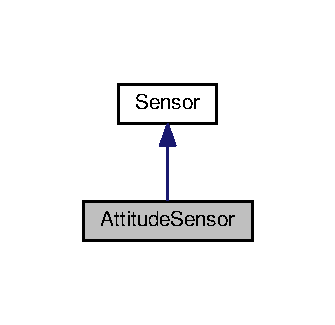
\includegraphics[width=161pt]{classAttitudeSensor__inherit__graph}
\end{center}
\end{figure}


Collaboration diagram for Attitude\+Sensor\+:\nopagebreak
\begin{figure}[H]
\begin{center}
\leavevmode
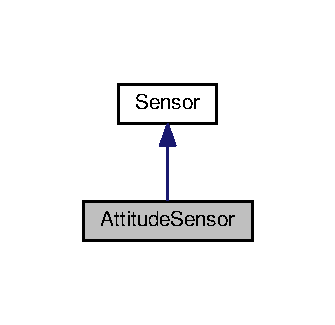
\includegraphics[width=161pt]{classAttitudeSensor__coll__graph}
\end{center}
\end{figure}
\subsection*{Public Member Functions}
\begin{DoxyCompactItemize}
\item 
{\bfseries Attitude\+Sensor} (int sensor\+Handle)\hypertarget{classAttitudeSensor_ada1382f003b390e357e9617e00299ddd}{}\label{classAttitudeSensor_ada1382f003b390e357e9617e00299ddd}

\item 
int \hyperlink{classAttitudeSensor_a354f56cfccea6f60b4822b9e2603afc8}{get} (std\+::vector$<$ float $>$ \&detect\+Angles)
\item 
void \hyperlink{classAttitudeSensor_a035c43c2ae16df0dedbbc7ae4cb575d9}{update} (std\+::vector$<$ float $>$ \&f, int \&i, std\+::vector$<$ float $>$ \&ff)
\item 
int \hyperlink{classAttitudeSensor_a29d069767d7b3b36a998ae70764134dd}{get} (std\+::vector$<$ float $>$ \&detect\+Point, int \&detect\+Handle, std\+::vector$<$ float $>$ \&detect\+Surface)
\end{DoxyCompactItemize}
\subsection*{Additional Inherited Members}


\subsection{Detailed Description}
currently unused class for an attitude sensor. currently the attitude is grabbed directly from the copter base object in vrep (which is the same as would be done in this class with more overhead) may be extended for use later for extending sensor functionality, e.\+g. implementing inaccuacies and noise 

\subsection{Member Function Documentation}
\index{Attitude\+Sensor@{Attitude\+Sensor}!get@{get}}
\index{get@{get}!Attitude\+Sensor@{Attitude\+Sensor}}
\subsubsection[{\texorpdfstring{get(std\+::vector$<$ float $>$ \&detect\+Angles)}{get(std::vector< float > &detectAngles)}}]{\setlength{\rightskip}{0pt plus 5cm}int Attitude\+Sensor\+::get (
\begin{DoxyParamCaption}
\item[{std\+::vector$<$ float $>$ \&}]{vfloat}
\end{DoxyParamCaption}
)\hspace{0.3cm}{\ttfamily [virtual]}}\hypertarget{classAttitudeSensor_a354f56cfccea6f60b4822b9e2603afc8}{}\label{classAttitudeSensor_a354f56cfccea6f60b4822b9e2603afc8}
retrieves the sensor information, limited to the position of a detected object; see specific sensor documentation for parameter information 

Implements \hyperlink{classSensor_a24f11619b11d5effc4066546629179ae}{Sensor}.

\index{Attitude\+Sensor@{Attitude\+Sensor}!get@{get}}
\index{get@{get}!Attitude\+Sensor@{Attitude\+Sensor}}
\subsubsection[{\texorpdfstring{get(std\+::vector$<$ float $>$ \&detect\+Point, int \&detect\+Handle, std\+::vector$<$ float $>$ \&detect\+Surface)}{get(std::vector< float > &detectPoint, int &detectHandle, std::vector< float > &detectSurface)}}]{\setlength{\rightskip}{0pt plus 5cm}int Attitude\+Sensor\+::get (
\begin{DoxyParamCaption}
\item[{std\+::vector$<$ float $>$ \&}]{detect\+Point, }
\item[{int \&}]{detect\+Handle, }
\item[{std\+::vector$<$ float $>$ \&}]{detect\+Surface}
\end{DoxyParamCaption}
)\hspace{0.3cm}{\ttfamily [virtual]}}\hypertarget{classAttitudeSensor_a29d069767d7b3b36a998ae70764134dd}{}\label{classAttitudeSensor_a29d069767d7b3b36a998ae70764134dd}
retrieves the sensor information, including any detected object information; see specific sensor documentation for paramter information 

Implements \hyperlink{classSensor_a997a8679d48c4fa346e6ac43c1e6219a}{Sensor}.

\index{Attitude\+Sensor@{Attitude\+Sensor}!update@{update}}
\index{update@{update}!Attitude\+Sensor@{Attitude\+Sensor}}
\subsubsection[{\texorpdfstring{update(std\+::vector$<$ float $>$ \&f, int \&i, std\+::vector$<$ float $>$ \&ff)}{update(std::vector< float > &f, int &i, std::vector< float > &ff)}}]{\setlength{\rightskip}{0pt plus 5cm}void Attitude\+Sensor\+::update (
\begin{DoxyParamCaption}
\item[{std\+::vector$<$ float $>$ \&}]{f, }
\item[{int \&}]{i, }
\item[{std\+::vector$<$ float $>$ \&}]{ff}
\end{DoxyParamCaption}
)\hspace{0.3cm}{\ttfamily [virtual]}}\hypertarget{classAttitudeSensor_a035c43c2ae16df0dedbbc7ae4cb575d9}{}\label{classAttitudeSensor_a035c43c2ae16df0dedbbc7ae4cb575d9}
calls for Vrep to update the sensor information; see specific sensor documentation for parameter information 

Implements \hyperlink{classSensor_abb6c93c88529bc392d129443b3d352f3}{Sensor}.



The documentation for this class was generated from the following files\+:\begin{DoxyCompactItemize}
\item 
attitudesensor.\+h\item 
attitudesensor.\+cpp\end{DoxyCompactItemize}

\hypertarget{structecef__coords}{}\section{ecef\+\_\+coords Struct Reference}
\label{structecef__coords}\index{ecef\+\_\+coords@{ecef\+\_\+coords}}
\subsection*{Public Attributes}
\begin{DoxyCompactItemize}
\item 
float {\bfseries x} = 3862.\+7\hypertarget{structecef__coords_a8babce644114c7da9a19e637baa121d3}{}\label{structecef__coords_a8babce644114c7da9a19e637baa121d3}

\item 
float {\bfseries y} = 750.\+8\hypertarget{structecef__coords_a1d7a58480890290b44784ebee21db0fa}{}\label{structecef__coords_a1d7a58480890290b44784ebee21db0fa}

\item 
float {\bfseries z} = 5002.\+8\hypertarget{structecef__coords_a7c8f017506769d9e7ebe1115b62e56bb}{}\label{structecef__coords_a7c8f017506769d9e7ebe1115b62e56bb}

\end{DoxyCompactItemize}


The documentation for this struct was generated from the following file\+:\begin{DoxyCompactItemize}
\item 
finken.\+cpp\end{DoxyCompactItemize}

\hypertarget{classFinken}{}\section{Finken Class Reference}
\label{classFinken}\index{Finken@{Finken}}


{\ttfamily \#include $<$finken.\+h$>$}

\subsection*{Public Member Functions}
\begin{DoxyCompactItemize}
\item 
\hyperlink{classFinken_afb256567ee9aa96c409fdb0529b4f228}{Finken} ()
\item 
\hyperlink{classFinken_a26a9cd42385ec3ae010e2ad1387d9ce6}{Finken} (int f\+Handle, int \+\_\+ac\+\_\+id, int \hyperlink{classFinken_a2de6be70e0baaf63641df0214bf1f7a2}{rotor\+Count}, int sonar\+Count)
\item 
\hyperlink{classFinken_a94e6a3b5b14ec7ee351d219eb17be45b}{$\sim$\+Finken} ()
\item 
void \hyperlink{classFinken_aa4779668e3bf85253e371b30e0da808a}{connect} (std\+::unique\+\_\+ptr$<$ tcp\+::iostream $>$ \&\&s\+Ptr)
\item 
void \hyperlink{classFinken_ae3c3abbf571407e210f4b03b68cada9d}{run} (std\+::unique\+\_\+ptr$<$ tcp\+::iostream $>$ s\+Ptr)
\item 
void \hyperlink{classFinken_aaead1098c0752c8ec5b99bccd9945f3b}{set\+Rotor\+Speeds} ()
\item 
void \hyperlink{classFinken_afddc56af42f000ff17c4a00779b4ad6a}{update\+Pos} (\hyperlink{classFinken}{Finken} \&finken)
\item 
std\+::vector$<$ std\+::unique\+\_\+ptr$<$ \hyperlink{classSensor}{Sensor} $>$ $>$ \& \hyperlink{classFinken_a1215883fb6df7c4853e498dec43b4e6a}{get\+Sensors} ()
\item 
std\+::vector$<$ std\+::unique\+\_\+ptr$<$ \hyperlink{classRotor}{Rotor} $>$ $>$ \& \hyperlink{classFinken_a610ce496f1c5f2ca22850ee26c54510c}{get\+Rotors} ()
\end{DoxyCompactItemize}
\begin{Indent}{\bf Construction functions}\par
{\em Functions needed to construct the copter in the vrep plugin \begin{DoxySeeAlso}{See also}
\hyperlink{finken_8cpp_ab8920c514423348469521fe0063534c4}{build\+Finken()} 
\end{DoxySeeAlso}
}\begin{DoxyCompactItemize}
\item 
void \hyperlink{classFinken_a2f2adb211e80a689f580b87730aeb9d1}{add\+Sensor} (std\+::unique\+\_\+ptr$<$ \hyperlink{classSensor}{Sensor} $>$ \&sensor)
\item 
void \hyperlink{classFinken_a4ac9d9b37fba41147a83a36286fbe91b}{add\+Rotor} (std\+::unique\+\_\+ptr$<$ \hyperlink{classRotor}{Rotor} $>$ \&rotor)
\end{DoxyCompactItemize}
\end{Indent}
\subsection*{Public Attributes}
\begin{DoxyCompactItemize}
\item 
int \hyperlink{classFinken_a96990553bc26c8bf26effe8edd6e6369}{handle}
\item 
int \hyperlink{classFinken_aef4736605ea21831e5340f66a931f8ac}{base\+Handle}
\item 
const int \hyperlink{classFinken_a496f5024f0876710ca1cfd55a2924e85}{ac\+\_\+id}
\item 
const int \hyperlink{classFinken_a2de6be70e0baaf63641df0214bf1f7a2}{rotor\+Count}
\item 
bool \hyperlink{classFinken_a83131e08852cbcebaffa1eef80164a6e}{connected} = 0
\item 
std\+::thread {\bfseries run\+Thread}\hypertarget{classFinken_a490f025c596b5c87d1c583124b53e34b}{}\label{classFinken_a490f025c596b5c87d1c583124b53e34b}

\item 
std\+::vector$<$ double $>$ \hyperlink{classFinken_aa4fe546d88b52ff92990bd67ced70567}{commands} = \{0,0,0,0\}
\end{DoxyCompactItemize}
\begin{Indent}{\bf Copter state}\par
{\em \label{classFinken_copterstate}%
\hypertarget{classFinken_copterstate}{}%
 Members representing the current copter state }\begin{DoxyCompactItemize}
\item 
std\+::vector$<$ double $>$ \hyperlink{classFinken_a726c0ea1d756fe0837a3f042665d8d4a}{pos} = \{-\/1,-\/1,-\/1\}
\item 
std\+::vector$<$ double $>$ \hyperlink{classFinken_a3968cbe3b6f76678367ecb61f044a221}{quat} = \{-\/1,-\/1,-\/1,-\/1\}
\item 
std\+::vector$<$ double $>$ \hyperlink{classFinken_a4dd260e6384e7cfb8040bd53fe1c2d62}{vel} = \{-\/1,-\/1,-\/1\}
\item 
std\+::vector$<$ double $>$ \hyperlink{classFinken_a518ab8ab8ac8cf54c0b79cbc1ec2075f}{rot\+Vel} =\{-\/1,-\/1,-\/1\}
\item 
std\+::vector$<$ double $>$ \hyperlink{classFinken_a6f9723479baee5573447036270a2a722}{accel} = \{-\/1,-\/1,-\/1\}
\item 
std\+::vector$<$ double $>$ \hyperlink{classFinken_ab1b738a1b691879be240b1b9488f7009}{rot\+Accel} =\{-\/1,-\/1,-\/1\}
\end{DoxyCompactItemize}
\end{Indent}


\subsection{Detailed Description}
\hyperlink{classFinken}{Finken} class for handling any data exchanges between a F\+I\+Nken and paparazzi. Also handles the application of rotor mixing commands to the F\+I\+Nken. 

\subsection{Constructor \& Destructor Documentation}
\index{Finken@{Finken}!Finken@{Finken}}
\index{Finken@{Finken}!Finken@{Finken}}
\subsubsection[{\texorpdfstring{Finken()}{Finken()}}]{\setlength{\rightskip}{0pt plus 5cm}Finken\+::\+Finken (
\begin{DoxyParamCaption}
{}
\end{DoxyParamCaption}
)}\hypertarget{classFinken_afb256567ee9aa96c409fdb0529b4f228}{}\label{classFinken_afb256567ee9aa96c409fdb0529b4f228}
Basic Empty Constructor \index{Finken@{Finken}!Finken@{Finken}}
\index{Finken@{Finken}!Finken@{Finken}}
\subsubsection[{\texorpdfstring{Finken(int f\+Handle, int \+\_\+ac\+\_\+id, int rotor\+Count, int sonar\+Count)}{Finken(int fHandle, int _ac_id, int rotorCount, int sonarCount)}}]{\setlength{\rightskip}{0pt plus 5cm}Finken\+::\+Finken (
\begin{DoxyParamCaption}
\item[{int}]{f\+Handle, }
\item[{int}]{\+\_\+ac\+\_\+id, }
\item[{int}]{rotor\+Count, }
\item[{int}]{sonar\+Count}
\end{DoxyParamCaption}
)}\hypertarget{classFinken_a26a9cd42385ec3ae010e2ad1387d9ce6}{}\label{classFinken_a26a9cd42385ec3ae010e2ad1387d9ce6}
Constructor for creating a uniquely identifiable finken 
\begin{DoxyParams}{Parameters}
{\em f\+Handle} & the handle used to identify the finken in vrep \\
\hline
{\em \+\_\+ac\+\_\+id} & the Aircraft ID used to identify the copter in paparazzi \\
\hline
\end{DoxyParams}
\index{Finken@{Finken}!````~Finken@{$\sim$\+Finken}}
\index{````~Finken@{$\sim$\+Finken}!Finken@{Finken}}
\subsubsection[{\texorpdfstring{$\sim$\+Finken()}{~Finken()}}]{\setlength{\rightskip}{0pt plus 5cm}Finken\+::$\sim$\+Finken (
\begin{DoxyParamCaption}
{}
\end{DoxyParamCaption}
)\hspace{0.3cm}{\ttfamily [inline]}}\hypertarget{classFinken_a94e6a3b5b14ec7ee351d219eb17be45b}{}\label{classFinken_a94e6a3b5b14ec7ee351d219eb17be45b}
Basic destructor 

\subsection{Member Function Documentation}
\index{Finken@{Finken}!add\+Rotor@{add\+Rotor}}
\index{add\+Rotor@{add\+Rotor}!Finken@{Finken}}
\subsubsection[{\texorpdfstring{add\+Rotor(std\+::unique\+\_\+ptr$<$ Rotor $>$ \&rotor)}{addRotor(std::unique_ptr< Rotor > &rotor)}}]{\setlength{\rightskip}{0pt plus 5cm}void Finken\+::add\+Rotor (
\begin{DoxyParamCaption}
\item[{std\+::unique\+\_\+ptr$<$ {\bf Rotor} $>$ \&}]{rotor}
\end{DoxyParamCaption}
)}\hypertarget{classFinken_a4ac9d9b37fba41147a83a36286fbe91b}{}\label{classFinken_a4ac9d9b37fba41147a83a36286fbe91b}
Adding rotors to the copter. \index{Finken@{Finken}!add\+Sensor@{add\+Sensor}}
\index{add\+Sensor@{add\+Sensor}!Finken@{Finken}}
\subsubsection[{\texorpdfstring{add\+Sensor(std\+::unique\+\_\+ptr$<$ Sensor $>$ \&sensor)}{addSensor(std::unique_ptr< Sensor > &sensor)}}]{\setlength{\rightskip}{0pt plus 5cm}void Finken\+::add\+Sensor (
\begin{DoxyParamCaption}
\item[{std\+::unique\+\_\+ptr$<$ {\bf Sensor} $>$ \&}]{sensor}
\end{DoxyParamCaption}
)}\hypertarget{classFinken_a2f2adb211e80a689f580b87730aeb9d1}{}\label{classFinken_a2f2adb211e80a689f580b87730aeb9d1}
Adding sensors to the copter. \index{Finken@{Finken}!connect@{connect}}
\index{connect@{connect}!Finken@{Finken}}
\subsubsection[{\texorpdfstring{connect(std\+::unique\+\_\+ptr$<$ tcp\+::iostream $>$ \&\&s\+Ptr)}{connect(std::unique_ptr< tcp::iostream > &&sPtr)}}]{\setlength{\rightskip}{0pt plus 5cm}void Finken\+::connect (
\begin{DoxyParamCaption}
\item[{std\+::unique\+\_\+ptr$<$ tcp\+::iostream $>$ \&\&}]{s\+Ptr}
\end{DoxyParamCaption}
)\hspace{0.3cm}{\ttfamily [inline]}}\hypertarget{classFinken_aa4779668e3bf85253e371b30e0da808a}{}\label{classFinken_aa4779668e3bf85253e371b30e0da808a}
Called in the accept handler, this function passes the incoming connection to the corresponding finken in a new thread \index{Finken@{Finken}!get\+Rotors@{get\+Rotors}}
\index{get\+Rotors@{get\+Rotors}!Finken@{Finken}}
\subsubsection[{\texorpdfstring{get\+Rotors()}{getRotors()}}]{\setlength{\rightskip}{0pt plus 5cm}std\+::vector$<$ std\+::unique\+\_\+ptr$<$ {\bf Rotor} $>$ $>$ \& Finken\+::get\+Rotors (
\begin{DoxyParamCaption}
{}
\end{DoxyParamCaption}
)}\hypertarget{classFinken_a610ce496f1c5f2ca22850ee26c54510c}{}\label{classFinken_a610ce496f1c5f2ca22850ee26c54510c}
returns a vector containing all rotors of the finken \index{Finken@{Finken}!get\+Sensors@{get\+Sensors}}
\index{get\+Sensors@{get\+Sensors}!Finken@{Finken}}
\subsubsection[{\texorpdfstring{get\+Sensors()}{getSensors()}}]{\setlength{\rightskip}{0pt plus 5cm}std\+::vector$<$ std\+::unique\+\_\+ptr$<$ {\bf Sensor} $>$ $>$ \& Finken\+::get\+Sensors (
\begin{DoxyParamCaption}
{}
\end{DoxyParamCaption}
)}\hypertarget{classFinken_a1215883fb6df7c4853e498dec43b4e6a}{}\label{classFinken_a1215883fb6df7c4853e498dec43b4e6a}
returns a vector containing all sensors of the finken \index{Finken@{Finken}!run@{run}}
\index{run@{run}!Finken@{Finken}}
\subsubsection[{\texorpdfstring{run(std\+::unique\+\_\+ptr$<$ tcp\+::iostream $>$ s\+Ptr)}{run(std::unique_ptr< tcp::iostream > sPtr)}}]{\setlength{\rightskip}{0pt plus 5cm}void Finken\+::run (
\begin{DoxyParamCaption}
\item[{std\+::unique\+\_\+ptr$<$ tcp\+::iostream $>$}]{s\+Ptr}
\end{DoxyParamCaption}
)}\hypertarget{classFinken_ae3c3abbf571407e210f4b03b68cada9d}{}\label{classFinken_ae3c3abbf571407e210f4b03b68cada9d}
Main function containing the paparazzi-\/vrep communication loop. Called whenever a new connection from paparazzi to the vrep server is established, see Async\+\_\+\+Server\+::handle\+\_\+accept() 
\begin{DoxyParams}{Parameters}
{\em s\+Ptr} & the iostream of the connection \\
\hline
\end{DoxyParams}
\begin{DoxySeeAlso}{See also}
Async\+\_\+\+Server\+::handle\+\_\+accept() 
\end{DoxySeeAlso}
\index{Finken@{Finken}!set\+Rotor\+Speeds@{set\+Rotor\+Speeds}}
\index{set\+Rotor\+Speeds@{set\+Rotor\+Speeds}!Finken@{Finken}}
\subsubsection[{\texorpdfstring{set\+Rotor\+Speeds()}{setRotorSpeeds()}}]{\setlength{\rightskip}{0pt plus 5cm}void Finken\+::set\+Rotor\+Speeds (
\begin{DoxyParamCaption}
{}
\end{DoxyParamCaption}
)}\hypertarget{classFinken_aaead1098c0752c8ec5b99bccd9945f3b}{}\label{classFinken_aaead1098c0752c8ec5b99bccd9945f3b}
Applies the correct rotor speeds calculated by paparazzi \begin{DoxySeeAlso}{See also}
\hyperlink{classFinken_aa4fe546d88b52ff92990bd67ced70567}{Finken\+::commands} 

\hyperlink{finken_8h_a4e838d73ad5e098825ef4c227f6369b6}{thrust\+From\+Throttle} 
\end{DoxySeeAlso}
\index{Finken@{Finken}!update\+Pos@{update\+Pos}}
\index{update\+Pos@{update\+Pos}!Finken@{Finken}}
\subsubsection[{\texorpdfstring{update\+Pos(\+Finken \&finken)}{updatePos(Finken &finken)}}]{\setlength{\rightskip}{0pt plus 5cm}void Finken\+::update\+Pos (
\begin{DoxyParamCaption}
\item[{{\bf Finken} \&}]{finken}
\end{DoxyParamCaption}
)}\hypertarget{classFinken_afddc56af42f000ff17c4a00779b4ad6a}{}\label{classFinken_afddc56af42f000ff17c4a00779b4ad6a}
updates the values for copter position and attitude, namely the \hyperlink{classFinken_copterstate}{copter state} vectors 
\begin{DoxyParams}{Parameters}
{\em finken} & reference to the finken to be updated \\
\hline
\end{DoxyParams}


\subsection{Member Data Documentation}
\index{Finken@{Finken}!ac\+\_\+id@{ac\+\_\+id}}
\index{ac\+\_\+id@{ac\+\_\+id}!Finken@{Finken}}
\subsubsection[{\texorpdfstring{ac\+\_\+id}{ac_id}}]{\setlength{\rightskip}{0pt plus 5cm}const int Finken\+::ac\+\_\+id}\hypertarget{classFinken_a496f5024f0876710ca1cfd55a2924e85}{}\label{classFinken_a496f5024f0876710ca1cfd55a2924e85}
Integer representing the Aircraft ID to match copters in vrep and paparazzi \index{Finken@{Finken}!accel@{accel}}
\index{accel@{accel}!Finken@{Finken}}
\subsubsection[{\texorpdfstring{accel}{accel}}]{\setlength{\rightskip}{0pt plus 5cm}std\+::vector$<$double$>$ Finken\+::accel = \{-\/1,-\/1,-\/1\}}\hypertarget{classFinken_a6f9723479baee5573447036270a2a722}{}\label{classFinken_a6f9723479baee5573447036270a2a722}
Copter acceleration \index{Finken@{Finken}!base\+Handle@{base\+Handle}}
\index{base\+Handle@{base\+Handle}!Finken@{Finken}}
\subsubsection[{\texorpdfstring{base\+Handle}{baseHandle}}]{\setlength{\rightskip}{0pt plus 5cm}int Finken\+::base\+Handle}\hypertarget{classFinken_aef4736605ea21831e5340f66a931f8ac}{}\label{classFinken_aef4736605ea21831e5340f66a931f8ac}
Integer representing the handle of the copter base in Vrep. Copter base, not the copter object is used for the calculation of the copter state. \index{Finken@{Finken}!commands@{commands}}
\index{commands@{commands}!Finken@{Finken}}
\subsubsection[{\texorpdfstring{commands}{commands}}]{\setlength{\rightskip}{0pt plus 5cm}std\+::vector$<$double$>$ Finken\+::commands = \{0,0,0,0\}}\hypertarget{classFinken_aa4fe546d88b52ff92990bd67ced70567}{}\label{classFinken_aa4fe546d88b52ff92990bd67ced70567}
Vector storing the commands provided by paparazzi \index{Finken@{Finken}!connected@{connected}}
\index{connected@{connected}!Finken@{Finken}}
\subsubsection[{\texorpdfstring{connected}{connected}}]{\setlength{\rightskip}{0pt plus 5cm}bool Finken\+::connected = 0}\hypertarget{classFinken_a83131e08852cbcebaffa1eef80164a6e}{}\label{classFinken_a83131e08852cbcebaffa1eef80164a6e}
Integer representing the amount for sonars, used in automatic finken construction$\ast$$\ast$ \begin{DoxySeeAlso}{See also}
\hyperlink{finken_8h_ab8920c514423348469521fe0063534c4}{build\+Finken} / const int sonar\+Count; /$\ast$$\ast$ current connection status of the copter 
\end{DoxySeeAlso}
\index{Finken@{Finken}!handle@{handle}}
\index{handle@{handle}!Finken@{Finken}}
\subsubsection[{\texorpdfstring{handle}{handle}}]{\setlength{\rightskip}{0pt plus 5cm}int Finken\+::handle}\hypertarget{classFinken_a96990553bc26c8bf26effe8edd6e6369}{}\label{classFinken_a96990553bc26c8bf26effe8edd6e6369}
Integer representing the handle of the copter object in vrep \index{Finken@{Finken}!pos@{pos}}
\index{pos@{pos}!Finken@{Finken}}
\subsubsection[{\texorpdfstring{pos}{pos}}]{\setlength{\rightskip}{0pt plus 5cm}std\+::vector$<$double$>$ Finken\+::pos = \{-\/1,-\/1,-\/1\}}\hypertarget{classFinken_a726c0ea1d756fe0837a3f042665d8d4a}{}\label{classFinken_a726c0ea1d756fe0837a3f042665d8d4a}
Copter position (E\+NU) \index{Finken@{Finken}!quat@{quat}}
\index{quat@{quat}!Finken@{Finken}}
\subsubsection[{\texorpdfstring{quat}{quat}}]{\setlength{\rightskip}{0pt plus 5cm}std\+::vector$<$double$>$ Finken\+::quat = \{-\/1,-\/1,-\/1,-\/1\}}\hypertarget{classFinken_a3968cbe3b6f76678367ecb61f044a221}{}\label{classFinken_a3968cbe3b6f76678367ecb61f044a221}
Copter Quaternion \index{Finken@{Finken}!rot\+Accel@{rot\+Accel}}
\index{rot\+Accel@{rot\+Accel}!Finken@{Finken}}
\subsubsection[{\texorpdfstring{rot\+Accel}{rotAccel}}]{\setlength{\rightskip}{0pt plus 5cm}std\+::vector$<$double$>$ Finken\+::rot\+Accel =\{-\/1,-\/1,-\/1\}}\hypertarget{classFinken_ab1b738a1b691879be240b1b9488f7009}{}\label{classFinken_ab1b738a1b691879be240b1b9488f7009}
Copter rotational acceleration (aka angular acceleration) \index{Finken@{Finken}!rotor\+Count@{rotor\+Count}}
\index{rotor\+Count@{rotor\+Count}!Finken@{Finken}}
\subsubsection[{\texorpdfstring{rotor\+Count}{rotorCount}}]{\setlength{\rightskip}{0pt plus 5cm}const int Finken\+::rotor\+Count}\hypertarget{classFinken_a2de6be70e0baaf63641df0214bf1f7a2}{}\label{classFinken_a2de6be70e0baaf63641df0214bf1f7a2}
Integer representing the amount for rotors, used in automatic finken construction \begin{DoxySeeAlso}{See also}
\hyperlink{finken_8cpp_ab8920c514423348469521fe0063534c4}{build\+Finken()} 
\end{DoxySeeAlso}
\index{Finken@{Finken}!rot\+Vel@{rot\+Vel}}
\index{rot\+Vel@{rot\+Vel}!Finken@{Finken}}
\subsubsection[{\texorpdfstring{rot\+Vel}{rotVel}}]{\setlength{\rightskip}{0pt plus 5cm}std\+::vector$<$double$>$ Finken\+::rot\+Vel =\{-\/1,-\/1,-\/1\}}\hypertarget{classFinken_a518ab8ab8ac8cf54c0b79cbc1ec2075f}{}\label{classFinken_a518ab8ab8ac8cf54c0b79cbc1ec2075f}
Copter rotational velocity (aka angular velocity) \index{Finken@{Finken}!vel@{vel}}
\index{vel@{vel}!Finken@{Finken}}
\subsubsection[{\texorpdfstring{vel}{vel}}]{\setlength{\rightskip}{0pt plus 5cm}std\+::vector$<$double$>$ Finken\+::vel = \{-\/1,-\/1,-\/1\}}\hypertarget{classFinken_a4dd260e6384e7cfb8040bd53fe1c2d62}{}\label{classFinken_a4dd260e6384e7cfb8040bd53fe1c2d62}
Copter velocity 

The documentation for this class was generated from the following files\+:\begin{DoxyCompactItemize}
\item 
\hyperlink{finken_8h}{finken.\+h}\item 
\hyperlink{finken_8cpp}{finken.\+cpp}\end{DoxyCompactItemize}

\hypertarget{classfinkenPID}{}\section{finken\+P\+ID Class Reference}
\label{classfinkenPID}\index{finken\+P\+ID@{finken\+P\+ID}}
\subsection*{Public Member Functions}
\begin{DoxyCompactItemize}
\item 
void {\bfseries init\+P\+ID} (float newP, float newI, float newD)\hypertarget{classfinkenPID_aeb81b68dad305019abbd9c17c641aeaf}{}\label{classfinkenPID_aeb81b68dad305019abbd9c17c641aeaf}

\item 
float {\bfseries step} (float newE, float deltaT)\hypertarget{classfinkenPID_a89d4d494967f124d0772accf90da38e5}{}\label{classfinkenPID_a89d4d494967f124d0772accf90da38e5}

\end{DoxyCompactItemize}
\subsection*{Public Attributes}
\begin{DoxyCompactItemize}
\item 
float {\bfseries p}\hypertarget{classfinkenPID_a571224b8b2987d6f9b66324b19d23a7a}{}\label{classfinkenPID_a571224b8b2987d6f9b66324b19d23a7a}

\item 
float {\bfseries i}\hypertarget{classfinkenPID_ae30f53812eb9ce918ff7118f1ed0bc37}{}\label{classfinkenPID_ae30f53812eb9ce918ff7118f1ed0bc37}

\item 
float {\bfseries d}\hypertarget{classfinkenPID_a6c2bc535c7059f44f221d7e439fff219}{}\label{classfinkenPID_a6c2bc535c7059f44f221d7e439fff219}

\item 
float {\bfseries e}\hypertarget{classfinkenPID_a072d0522c05093becbd516058ba50357}{}\label{classfinkenPID_a072d0522c05093becbd516058ba50357}

\item 
float {\bfseries e\+\_\+prev}\hypertarget{classfinkenPID_a8a489dbad77576f5e36056ab8d510ea8}{}\label{classfinkenPID_a8a489dbad77576f5e36056ab8d510ea8}

\item 
float {\bfseries e\+\_\+sum}\hypertarget{classfinkenPID_ab336cafd17c6979c9da52a722af5cd4f}{}\label{classfinkenPID_ab336cafd17c6979c9da52a722af5cd4f}

\end{DoxyCompactItemize}


The documentation for this class was generated from the following files\+:\begin{DoxyCompactItemize}
\item 
finken\+P\+I\+D.\+h\item 
finken\+P\+I\+D.\+cpp\end{DoxyCompactItemize}

\hypertarget{classFinkenPlugin}{}\section{Finken\+Plugin Class Reference}
\label{classFinkenPlugin}\index{Finken\+Plugin@{Finken\+Plugin}}


Inheritance diagram for Finken\+Plugin\+:\nopagebreak
\begin{figure}[H]
\begin{center}
\leavevmode
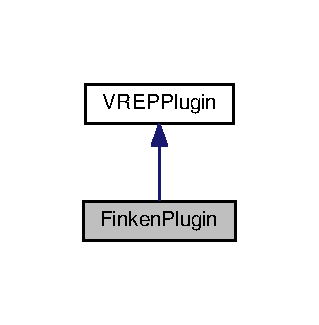
\includegraphics[width=153pt]{classFinkenPlugin__inherit__graph}
\end{center}
\end{figure}


Collaboration diagram for Finken\+Plugin\+:\nopagebreak
\begin{figure}[H]
\begin{center}
\leavevmode
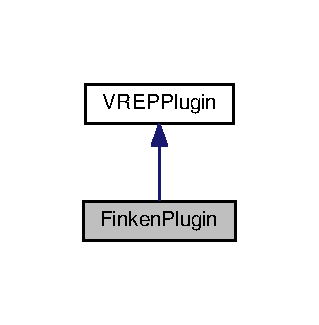
\includegraphics[width=153pt]{classFinkenPlugin__coll__graph}
\end{center}
\end{figure}
\subsection*{Public Member Functions}
\begin{DoxyCompactItemize}
\item 
\hyperlink{classFinkenPlugin}{Finken\+Plugin} \& {\bfseries operator=} (const \hyperlink{classFinkenPlugin}{Finken\+Plugin} \&)=delete\hypertarget{classFinkenPlugin_a3ebea1e19535491b5db16c7f43df8e79}{}\label{classFinkenPlugin_a3ebea1e19535491b5db16c7f43df8e79}

\item 
{\bfseries Finken\+Plugin} (const \hyperlink{classFinkenPlugin}{Finken\+Plugin} \&)=delete\hypertarget{classFinkenPlugin_a5f4bc33c0d0bb05ca4f78090c7a2fda9}{}\label{classFinkenPlugin_a5f4bc33c0d0bb05ca4f78090c7a2fda9}

\item 
virtual unsigned char {\bfseries version} () const \hypertarget{classFinkenPlugin_a046a229dfbc8185bac916ad2e49ec865}{}\label{classFinkenPlugin_a046a229dfbc8185bac916ad2e49ec865}

\item 
virtual bool \hyperlink{classFinkenPlugin_afbe5d82635afe4b0c407de4724e8ee14}{load} ()
\item 
virtual bool \hyperlink{classFinkenPlugin_ae9c984b362c6a828206fa6201291851c}{unload} ()
\item 
virtual const std\+::string {\bfseries name} () const \hypertarget{classFinkenPlugin_a1a7d0d65f88654c37b282e07d36417ec}{}\label{classFinkenPlugin_a1a7d0d65f88654c37b282e07d36417ec}

\item 
void $\ast$ \hyperlink{classFinkenPlugin_a82c0cd5fa1b9fdb5f5a625458a9b545b}{scene\+Load} (int $\ast$auxiliary\+Data, void $\ast$custom\+Data, int $\ast$reply\+Data)
\item 
void $\ast$ {\bfseries sim\+Start} (int $\ast$auxiliary\+Data, void $\ast$custom\+Data, int $\ast$reply\+Data)\hypertarget{classFinkenPlugin_a142f62305fcc926bb6cf86744edbb82b}{}\label{classFinkenPlugin_a142f62305fcc926bb6cf86744edbb82b}

\item 
void $\ast$ {\bfseries sim\+End} (int $\ast$auxiliary\+Data, void $\ast$custom\+Data, int $\ast$reply\+Data)\hypertarget{classFinkenPlugin_aec5f5cf14ca485055ccc321a716780a4}{}\label{classFinkenPlugin_aec5f5cf14ca485055ccc321a716780a4}

\item 
void $\ast$ \hyperlink{classFinkenPlugin_a00d8bcdd7c4b28eb76712b84f512b12b}{action} (int $\ast$auxiliary\+Data, void $\ast$custom\+Data, int $\ast$reply\+Data)
\end{DoxyCompactItemize}
\subsection*{Public Attributes}
\begin{DoxyCompactItemize}
\item 
boost\+::asio\+::io\+\_\+service \hyperlink{classFinkenPlugin_a895a0de924a1c60e3cb65ff1cf139fdc}{io\+\_\+service}
\item 
std\+::unique\+\_\+ptr$<$ \hyperlink{classAsync__Server}{Async\+\_\+\+Server} $>$ {\bfseries async\+\_\+server}\hypertarget{classFinkenPlugin_aeb198541b548eb5b1ba09221aaa35a26}{}\label{classFinkenPlugin_aeb198541b548eb5b1ba09221aaa35a26}

\end{DoxyCompactItemize}
\subsection*{Additional Inherited Members}


\subsection{Detailed Description}
The actual finken plugin. This class handles the main communication with vrep and calls for copter actions each timestep. It is also responsible for starting the server to communicate with paparazzi. 

\subsection{Member Function Documentation}
\index{Finken\+Plugin@{Finken\+Plugin}!action@{action}}
\index{action@{action}!Finken\+Plugin@{Finken\+Plugin}}
\subsubsection[{\texorpdfstring{action(int $\ast$auxiliary\+Data, void $\ast$custom\+Data, int $\ast$reply\+Data)}{action(int *auxiliaryData, void *customData, int *replyData)}}]{\setlength{\rightskip}{0pt plus 5cm}void$\ast$ Finken\+Plugin\+::action (
\begin{DoxyParamCaption}
\item[{int $\ast$}]{auxiliary\+Data, }
\item[{void $\ast$}]{custom\+Data, }
\item[{int $\ast$}]{reply\+Data}
\end{DoxyParamCaption}
)\hspace{0.3cm}{\ttfamily [inline]}, {\ttfamily [virtual]}}\hypertarget{classFinkenPlugin_a00d8bcdd7c4b28eb76712b84f512b12b}{}\label{classFinkenPlugin_a00d8bcdd7c4b28eb76712b84f512b12b}
This function controls the other parts of the plugin and synchronizes the vrep copters with the paparazzi copters. 

Reimplemented from \hyperlink{classVREPPlugin}{V\+R\+E\+P\+Plugin}.

\index{Finken\+Plugin@{Finken\+Plugin}!load@{load}}
\index{load@{load}!Finken\+Plugin@{Finken\+Plugin}}
\subsubsection[{\texorpdfstring{load()}{load()}}]{\setlength{\rightskip}{0pt plus 5cm}virtual bool Finken\+Plugin\+::load (
\begin{DoxyParamCaption}
{}
\end{DoxyParamCaption}
)\hspace{0.3cm}{\ttfamily [inline]}, {\ttfamily [virtual]}}\hypertarget{classFinkenPlugin_afbe5d82635afe4b0c407de4724e8ee14}{}\label{classFinkenPlugin_afbe5d82635afe4b0c407de4724e8ee14}
loads the plugin into vrep 

Reimplemented from \hyperlink{classVREPPlugin}{V\+R\+E\+P\+Plugin}.

\index{Finken\+Plugin@{Finken\+Plugin}!scene\+Load@{scene\+Load}}
\index{scene\+Load@{scene\+Load}!Finken\+Plugin@{Finken\+Plugin}}
\subsubsection[{\texorpdfstring{scene\+Load(int $\ast$auxiliary\+Data, void $\ast$custom\+Data, int $\ast$reply\+Data)}{sceneLoad(int *auxiliaryData, void *customData, int *replyData)}}]{\setlength{\rightskip}{0pt plus 5cm}void$\ast$ Finken\+Plugin\+::scene\+Load (
\begin{DoxyParamCaption}
\item[{int $\ast$}]{auxiliary\+Data, }
\item[{void $\ast$}]{custom\+Data, }
\item[{int $\ast$}]{reply\+Data}
\end{DoxyParamCaption}
)\hspace{0.3cm}{\ttfamily [inline]}, {\ttfamily [virtual]}}\hypertarget{classFinkenPlugin_a82c0cd5fa1b9fdb5f5a625458a9b545b}{}\label{classFinkenPlugin_a82c0cd5fa1b9fdb5f5a625458a9b545b}
Called once on the loading of any scene, it checks for the presence of a Dummy object \char`\"{}\+Script\+Loader\char`\"{} in the scene. Only if that object is found, the server is startet and full functionality established. 

Reimplemented from \hyperlink{classVREPPlugin}{V\+R\+E\+P\+Plugin}.

\index{Finken\+Plugin@{Finken\+Plugin}!unload@{unload}}
\index{unload@{unload}!Finken\+Plugin@{Finken\+Plugin}}
\subsubsection[{\texorpdfstring{unload()}{unload()}}]{\setlength{\rightskip}{0pt plus 5cm}virtual bool Finken\+Plugin\+::unload (
\begin{DoxyParamCaption}
{}
\end{DoxyParamCaption}
)\hspace{0.3cm}{\ttfamily [inline]}, {\ttfamily [virtual]}}\hypertarget{classFinkenPlugin_ae9c984b362c6a828206fa6201291851c}{}\label{classFinkenPlugin_ae9c984b362c6a828206fa6201291851c}
unloads the plugin 

Reimplemented from \hyperlink{classVREPPlugin}{V\+R\+E\+P\+Plugin}.



\subsection{Member Data Documentation}
\index{Finken\+Plugin@{Finken\+Plugin}!io\+\_\+service@{io\+\_\+service}}
\index{io\+\_\+service@{io\+\_\+service}!Finken\+Plugin@{Finken\+Plugin}}
\subsubsection[{\texorpdfstring{io\+\_\+service}{io_service}}]{\setlength{\rightskip}{0pt plus 5cm}boost\+::asio\+::io\+\_\+service Finken\+Plugin\+::io\+\_\+service}\hypertarget{classFinkenPlugin_a895a0de924a1c60e3cb65ff1cf139fdc}{}\label{classFinkenPlugin_a895a0de924a1c60e3cb65ff1cf139fdc}
The io service for the server 

The documentation for this class was generated from the following file\+:\begin{DoxyCompactItemize}
\item 
finkenplugin.\+cpp\end{DoxyCompactItemize}

\hypertarget{classHeightSensor}{}\section{Height\+Sensor Class Reference}
\label{classHeightSensor}\index{Height\+Sensor@{Height\+Sensor}}


{\ttfamily \#include $<$heightsensor.\+h$>$}



Inheritance diagram for Height\+Sensor\+:\nopagebreak
\begin{figure}[H]
\begin{center}
\leavevmode
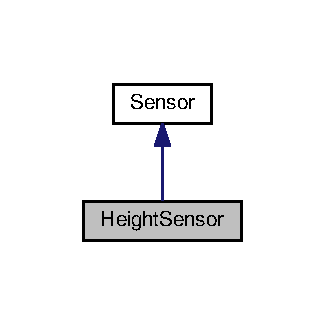
\includegraphics[width=156pt]{classHeightSensor__inherit__graph}
\end{center}
\end{figure}


Collaboration diagram for Height\+Sensor\+:\nopagebreak
\begin{figure}[H]
\begin{center}
\leavevmode
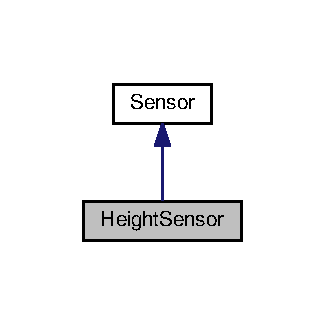
\includegraphics[width=156pt]{classHeightSensor__coll__graph}
\end{center}
\end{figure}
\subsection*{Public Member Functions}
\begin{DoxyCompactItemize}
\item 
{\bfseries Height\+Sensor} (int sensor\+Handle)\hypertarget{classHeightSensor_adce900c49d253c6e9cd85db00c2f0708}{}\label{classHeightSensor_adce900c49d253c6e9cd85db00c2f0708}

\item 
int \hyperlink{classHeightSensor_abd4b7d4cc5906a971da402757989f5da}{get} (std\+::vector$<$ float $>$ \&detect\+Point, int \&detect\+Handle, std\+::vector$<$ float $>$ \&detect\+Surface)
\item 
int \hyperlink{classHeightSensor_a90a19e600e5b89a503366da0f0c35590}{get} (std\+::vector$<$ float $>$ \&detect\+Point)
\item 
void \hyperlink{classHeightSensor_a6966090886a414a6213125c91a31e128}{update} (std\+::vector$<$ float $>$ \&f, int \&i, std\+::vector$<$ float $>$ \&ff)
\end{DoxyCompactItemize}
\subsection*{Additional Inherited Members}


\subsection{Detailed Description}
Class implementing a heightsensor 

\subsection{Member Function Documentation}
\index{Height\+Sensor@{Height\+Sensor}!get@{get}}
\index{get@{get}!Height\+Sensor@{Height\+Sensor}}
\subsubsection[{\texorpdfstring{get(std\+::vector$<$ float $>$ \&detect\+Point, int \&detect\+Handle, std\+::vector$<$ float $>$ \&detect\+Surface)}{get(std::vector< float > &detectPoint, int &detectHandle, std::vector< float > &detectSurface)}}]{\setlength{\rightskip}{0pt plus 5cm}int Height\+Sensor\+::get (
\begin{DoxyParamCaption}
\item[{std\+::vector$<$ float $>$ \&}]{detect\+Point, }
\item[{int \&}]{detect\+Handle, }
\item[{std\+::vector$<$ float $>$ \&}]{detect\+Surface}
\end{DoxyParamCaption}
)\hspace{0.3cm}{\ttfamily [virtual]}}\hypertarget{classHeightSensor_abd4b7d4cc5906a971da402757989f5da}{}\label{classHeightSensor_abd4b7d4cc5906a971da402757989f5da}
simply reads the sensor information with no additional call to handle the sensor in vrep 
\begin{DoxyParams}{Parameters}
{\em \&detect\+Point} & vector reference to store the coordinates of the closest point \\
\hline
{\em \&detect\+Handle} & integer reference to store the handle of the found object \\
\hline
{\em \&detect\+Surface} & vector reference to store the normal vector of the detected surface \\
\hline
\end{DoxyParams}


Implements \hyperlink{classSensor_a997a8679d48c4fa346e6ac43c1e6219a}{Sensor}.

\index{Height\+Sensor@{Height\+Sensor}!get@{get}}
\index{get@{get}!Height\+Sensor@{Height\+Sensor}}
\subsubsection[{\texorpdfstring{get(std\+::vector$<$ float $>$ \&detect\+Point)}{get(std::vector< float > &detectPoint)}}]{\setlength{\rightskip}{0pt plus 5cm}int Height\+Sensor\+::get (
\begin{DoxyParamCaption}
\item[{std\+::vector$<$ float $>$ \&}]{detect\+Point}
\end{DoxyParamCaption}
)\hspace{0.3cm}{\ttfamily [virtual]}}\hypertarget{classHeightSensor_a90a19e600e5b89a503366da0f0c35590}{}\label{classHeightSensor_a90a19e600e5b89a503366da0f0c35590}
same as the previous get, but all parameters except the coordinates of a detected point are omitted 

Implements \hyperlink{classSensor_a24f11619b11d5effc4066546629179ae}{Sensor}.

\index{Height\+Sensor@{Height\+Sensor}!update@{update}}
\index{update@{update}!Height\+Sensor@{Height\+Sensor}}
\subsubsection[{\texorpdfstring{update(std\+::vector$<$ float $>$ \&f, int \&i, std\+::vector$<$ float $>$ \&ff)}{update(std::vector< float > &f, int &i, std::vector< float > &ff)}}]{\setlength{\rightskip}{0pt plus 5cm}void Height\+Sensor\+::update (
\begin{DoxyParamCaption}
\item[{std\+::vector$<$ float $>$ \&}]{detect\+Point, }
\item[{int \&}]{detect\+Handle, }
\item[{std\+::vector$<$ float $>$ \&}]{detect\+Surface}
\end{DoxyParamCaption}
)\hspace{0.3cm}{\ttfamily [virtual]}}\hypertarget{classHeightSensor_a6966090886a414a6213125c91a31e128}{}\label{classHeightSensor_a6966090886a414a6213125c91a31e128}
calls for vrep to update the sensor information 
\begin{DoxyParams}{Parameters}
{\em \&detect\+Point} & vector reference to store the coordinates of the closest point \\
\hline
{\em \&detect\+Handle} & integer reference to store the handle of the found object \\
\hline
{\em \&detect\+Surface} & vector reference to store the normal vector of the detected surface \\
\hline
\end{DoxyParams}


Implements \hyperlink{classSensor_abb6c93c88529bc392d129443b3d352f3}{Sensor}.



The documentation for this class was generated from the following files\+:\begin{DoxyCompactItemize}
\item 
heightsensor.\+h\item 
heightsensor.\+cpp\end{DoxyCompactItemize}

\hypertarget{structlla__coords}{}\section{lla\+\_\+coords Struct Reference}
\label{structlla__coords}\index{lla\+\_\+coords@{lla\+\_\+coords}}
\subsection*{Public Attributes}
\begin{DoxyCompactItemize}
\item 
float {\bfseries lat} = 52\hypertarget{structlla__coords_a1c1072469e8272e10fba298c2a21656c}{}\label{structlla__coords_a1c1072469e8272e10fba298c2a21656c}

\item 
float {\bfseries lon} = 11\hypertarget{structlla__coords_a28ccc6c3e258a13b931102479a81d309}{}\label{structlla__coords_a28ccc6c3e258a13b931102479a81d309}

\item 
float {\bfseries height} = 50\hypertarget{structlla__coords_abdc3be56573ef86b19d3e4638558f1f2}{}\label{structlla__coords_abdc3be56573ef86b19d3e4638558f1f2}

\end{DoxyCompactItemize}


The documentation for this struct was generated from the following file\+:\begin{DoxyCompactItemize}
\item 
finken.\+cpp\end{DoxyCompactItemize}

\hypertarget{classLog}{}\section{Log Class Reference}
\label{classLog}\index{Log@{Log}}
\subsection*{Static Public Member Functions}
\begin{DoxyCompactItemize}
\item 
static const std\+::ostream \& {\bfseries out\+Stream} ()\hypertarget{classLog_a27b116b095e6e08d5e40fd365210c657}{}\label{classLog_a27b116b095e6e08d5e40fd365210c657}

\item 
static void {\bfseries out\+Stream} (std\+::ostream \&stream)\hypertarget{classLog_ad5a9c8a9d7f84d36041f21058f450e53}{}\label{classLog_ad5a9c8a9d7f84d36041f21058f450e53}

\item 
static const std\+::ostream \& {\bfseries err\+Stream} ()\hypertarget{classLog_ac209747fd4964bc121818481ee131d19}{}\label{classLog_ac209747fd4964bc121818481ee131d19}

\item 
static void {\bfseries err\+Stream} (std\+::ostream \&stream)\hypertarget{classLog_ab2c566571ace5d3f234707ddfaaed4c9}{}\label{classLog_ab2c566571ace5d3f234707ddfaaed4c9}

\item 
static const std\+::string \& {\bfseries name} ()\hypertarget{classLog_a5a4518f9758b1eee0adcac1c3119288b}{}\label{classLog_a5a4518f9758b1eee0adcac1c3119288b}

\item 
static void {\bfseries name} (const std\+::string \&name)\hypertarget{classLog_a5758fde0052d1b682c6e2a33be192ecd}{}\label{classLog_a5758fde0052d1b682c6e2a33be192ecd}

\item 
static std\+::ostream \& {\bfseries out} ()\hypertarget{classLog_ab89f6644dd040b1fa07c1253cc12bafb}{}\label{classLog_ab89f6644dd040b1fa07c1253cc12bafb}

\item 
static std\+::ostream \& {\bfseries err} ()\hypertarget{classLog_ad37da894b6f997bc5204ed81cace26c2}{}\label{classLog_ad37da894b6f997bc5204ed81cace26c2}

\end{DoxyCompactItemize}


The documentation for this class was generated from the following files\+:\begin{DoxyCompactItemize}
\item 
log.\+h\item 
log.\+cpp\end{DoxyCompactItemize}

\hypertarget{classLogLine}{}\section{Log\+Line Class Reference}
\label{classLogLine}\index{Log\+Line@{Log\+Line}}


{\ttfamily \#include $<$finken.\+h$>$}

\subsection*{Public Member Functions}
\begin{DoxyCompactItemize}
\item 
{\bfseries Log\+Line} (std\+::ostream \&o)\hypertarget{classLogLine_a7f1c876fef642fffb06f646749662a04}{}\label{classLogLine_a7f1c876fef642fffb06f646749662a04}

\item 
\hyperlink{classLogLine}{Log\+Line} \& {\bfseries operator$<$$<$} (std\+::ostream \&($\ast$pf)(std\+::ostream \&))\hypertarget{classLogLine_a9697d8126ee9dd2ee3ea70bc61abf4b8}{}\label{classLogLine_a9697d8126ee9dd2ee3ea70bc61abf4b8}

\item 
{\footnotesize template$<$typename T $>$ }\\\hyperlink{classLogLine}{Log\+Line} \& {\bfseries operator$<$$<$} (T t)\hypertarget{classLogLine_aa9dff12f0c1466e53e63f981872f1e76}{}\label{classLogLine_aa9dff12f0c1466e53e63f981872f1e76}

\end{DoxyCompactItemize}
\subsection*{Friends}
\begin{DoxyCompactItemize}
\item 
class {\bfseries Vrep\+Log}\hypertarget{classLogLine_a4b85b5c9be56c4b49e99130f36f2df1d}{}\label{classLogLine_a4b85b5c9be56c4b49e99130f36f2df1d}

\end{DoxyCompactItemize}


\subsection{Detailed Description}
Basic class for creating a log file 

The documentation for this class was generated from the following file\+:\begin{DoxyCompactItemize}
\item 
\hyperlink{finken_8h}{finken.\+h}\end{DoxyCompactItemize}

\hypertarget{classPositionSensor}{}\section{Position\+Sensor Class Reference}
\label{classPositionSensor}\index{Position\+Sensor@{Position\+Sensor}}


Inheritance diagram for Position\+Sensor\+:\nopagebreak
\begin{figure}[H]
\begin{center}
\leavevmode
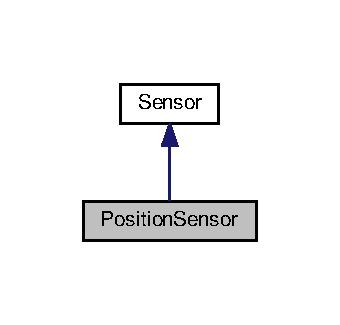
\includegraphics[width=163pt]{classPositionSensor__inherit__graph}
\end{center}
\end{figure}


Collaboration diagram for Position\+Sensor\+:\nopagebreak
\begin{figure}[H]
\begin{center}
\leavevmode
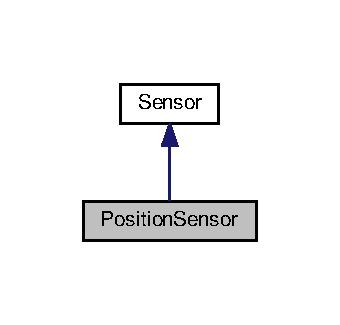
\includegraphics[width=163pt]{classPositionSensor__coll__graph}
\end{center}
\end{figure}
\subsection*{Public Member Functions}
\begin{DoxyCompactItemize}
\item 
{\bfseries Position\+Sensor} (int sensor\+Handle)\hypertarget{classPositionSensor_a1bc5cb93c92c04eef26d406dbb304ead}{}\label{classPositionSensor_a1bc5cb93c92c04eef26d406dbb304ead}

\item 
int \hyperlink{classPositionSensor_a99c4b37f9f16912b15603d79dda386bc}{get} (std\+::vector$<$ float $>$ \&detect\+Position)
\item 
void \hyperlink{classPositionSensor_a4fb083aa0462a73627b11b7c0e408f09}{update} (std\+::vector$<$ float $>$ \&f, int \&i, std\+::vector$<$ float $>$ \&ff)
\item 
int \hyperlink{classPositionSensor_a0b8c45d846d3442d94e2ef767fddf31d}{get} (std\+::vector$<$ float $>$ \&detect\+Point, int \&detect\+Handle, std\+::vector$<$ float $>$ \&detect\+Surface)
\end{DoxyCompactItemize}
\subsection*{Additional Inherited Members}


\subsection{Member Function Documentation}
\index{Position\+Sensor@{Position\+Sensor}!get@{get}}
\index{get@{get}!Position\+Sensor@{Position\+Sensor}}
\subsubsection[{\texorpdfstring{get(std\+::vector$<$ float $>$ \&detect\+Position)}{get(std::vector< float > &detectPosition)}}]{\setlength{\rightskip}{0pt plus 5cm}int Position\+Sensor\+::get (
\begin{DoxyParamCaption}
\item[{std\+::vector$<$ float $>$ \&}]{vfloat}
\end{DoxyParamCaption}
)\hspace{0.3cm}{\ttfamily [virtual]}}\hypertarget{classPositionSensor_a99c4b37f9f16912b15603d79dda386bc}{}\label{classPositionSensor_a99c4b37f9f16912b15603d79dda386bc}
retrieves the sensor information, limited to the position of a detected object; see specific sensor documentation for parameter information 

Implements \hyperlink{classSensor_a24f11619b11d5effc4066546629179ae}{Sensor}.

\index{Position\+Sensor@{Position\+Sensor}!get@{get}}
\index{get@{get}!Position\+Sensor@{Position\+Sensor}}
\subsubsection[{\texorpdfstring{get(std\+::vector$<$ float $>$ \&detect\+Point, int \&detect\+Handle, std\+::vector$<$ float $>$ \&detect\+Surface)}{get(std::vector< float > &detectPoint, int &detectHandle, std::vector< float > &detectSurface)}}]{\setlength{\rightskip}{0pt plus 5cm}int Position\+Sensor\+::get (
\begin{DoxyParamCaption}
\item[{std\+::vector$<$ float $>$ \&}]{detect\+Point, }
\item[{int \&}]{detect\+Handle, }
\item[{std\+::vector$<$ float $>$ \&}]{detect\+Surface}
\end{DoxyParamCaption}
)\hspace{0.3cm}{\ttfamily [virtual]}}\hypertarget{classPositionSensor_a0b8c45d846d3442d94e2ef767fddf31d}{}\label{classPositionSensor_a0b8c45d846d3442d94e2ef767fddf31d}
retrieves the sensor information, including any detected object information; see specific sensor documentation for paramter information 

Implements \hyperlink{classSensor_a997a8679d48c4fa346e6ac43c1e6219a}{Sensor}.

\index{Position\+Sensor@{Position\+Sensor}!update@{update}}
\index{update@{update}!Position\+Sensor@{Position\+Sensor}}
\subsubsection[{\texorpdfstring{update(std\+::vector$<$ float $>$ \&f, int \&i, std\+::vector$<$ float $>$ \&ff)}{update(std::vector< float > &f, int &i, std::vector< float > &ff)}}]{\setlength{\rightskip}{0pt plus 5cm}void Position\+Sensor\+::update (
\begin{DoxyParamCaption}
\item[{std\+::vector$<$ float $>$ \&}]{f, }
\item[{int \&}]{i, }
\item[{std\+::vector$<$ float $>$ \&}]{ff}
\end{DoxyParamCaption}
)\hspace{0.3cm}{\ttfamily [virtual]}}\hypertarget{classPositionSensor_a4fb083aa0462a73627b11b7c0e408f09}{}\label{classPositionSensor_a4fb083aa0462a73627b11b7c0e408f09}
calls for Vrep to update the sensor information; see specific sensor documentation for parameter information 

Implements \hyperlink{classSensor_abb6c93c88529bc392d129443b3d352f3}{Sensor}.



The documentation for this class was generated from the following files\+:\begin{DoxyCompactItemize}
\item 
positionsensor.\+h\item 
positionsensor.\+cpp\end{DoxyCompactItemize}

\hypertarget{classRotor}{}\section{Rotor Class Reference}
\label{classRotor}\index{Rotor@{Rotor}}
\subsection*{Public Member Functions}
\begin{DoxyCompactItemize}
\item 
{\bfseries Rotor} (int r\+Handle)\hypertarget{classRotor_ab1ad46cf401db508602fb136f09094c2}{}\label{classRotor_ab1ad46cf401db508602fb136f09094c2}

\item 
void {\bfseries set} (const std\+::vector$<$ float $>$ \&force, const std\+::vector$<$ float $>$ \&torque)\hypertarget{classRotor_aa961955180593d6249b3c35730b29cfb}{}\label{classRotor_aa961955180593d6249b3c35730b29cfb}

\end{DoxyCompactItemize}
\subsection*{Public Attributes}
\begin{DoxyCompactItemize}
\item 
int {\bfseries handle}\hypertarget{classRotor_ae6da9102b10f4759201a62117f6b2b6e}{}\label{classRotor_ae6da9102b10f4759201a62117f6b2b6e}

\end{DoxyCompactItemize}


The documentation for this class was generated from the following files\+:\begin{DoxyCompactItemize}
\item 
rotor.\+h\item 
rotor.\+cpp\end{DoxyCompactItemize}

\hypertarget{classSensor}{}\section{Sensor Class Reference}
\label{classSensor}\index{Sensor@{Sensor}}


{\ttfamily \#include $<$sensor.\+h$>$}



Inheritance diagram for Sensor\+:\nopagebreak
\begin{figure}[H]
\begin{center}
\leavevmode
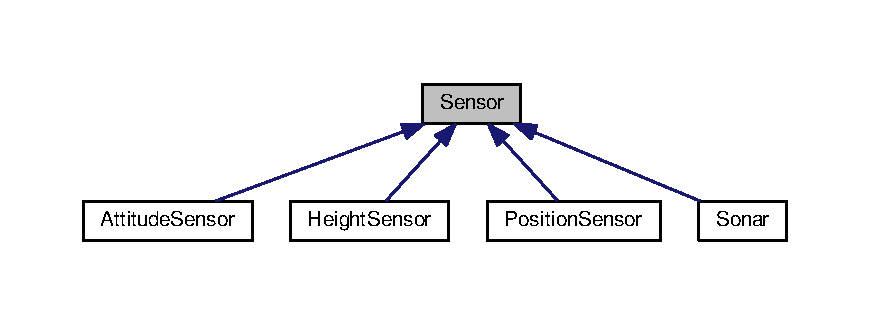
\includegraphics[width=350pt]{classSensor__inherit__graph}
\end{center}
\end{figure}
\subsection*{Public Member Functions}
\begin{DoxyCompactItemize}
\item 
\hyperlink{classSensor_aec15220e0b38da37e43b0525ac689499}{Sensor} (int sensor\+Handle)
\item 
virtual void \hyperlink{classSensor_abb6c93c88529bc392d129443b3d352f3}{update} (std\+::vector$<$ float $>$ \&f, int \&i, std\+::vector$<$ float $>$ \&ff)=0
\item 
virtual int \hyperlink{classSensor_a997a8679d48c4fa346e6ac43c1e6219a}{get} (std\+::vector$<$ float $>$ \&detect\+Point, int \&detect\+Handle, std\+::vector$<$ float $>$ \&detect\+Surface)=0
\item 
virtual int \hyperlink{classSensor_a24f11619b11d5effc4066546629179ae}{get} (std\+::vector$<$ float $>$ \&vfloat)=0
\item 
virtual int {\bfseries get\+Handle} ()\hypertarget{classSensor_ac647e98897da5ffcc9711ba27ec45abd}{}\label{classSensor_ac647e98897da5ffcc9711ba27ec45abd}

\end{DoxyCompactItemize}
\subsection*{Protected Attributes}
\begin{DoxyCompactItemize}
\item 
int \hyperlink{classSensor_ad31f2503e8a1cc7888e5eefbeede8f3b}{handle}
\end{DoxyCompactItemize}


\subsection{Detailed Description}
Basic \hyperlink{classSensor}{Sensor} class from which specialized sensors are derived 

\subsection{Constructor \& Destructor Documentation}
\index{Sensor@{Sensor}!Sensor@{Sensor}}
\index{Sensor@{Sensor}!Sensor@{Sensor}}
\subsubsection[{\texorpdfstring{Sensor(int sensor\+Handle)}{Sensor(int sensorHandle)}}]{\setlength{\rightskip}{0pt plus 5cm}Sensor\+::\+Sensor (
\begin{DoxyParamCaption}
\item[{int}]{sensor\+Handle}
\end{DoxyParamCaption}
)}\hypertarget{classSensor_aec15220e0b38da37e43b0525ac689499}{}\label{classSensor_aec15220e0b38da37e43b0525ac689499}
Constructor 
\begin{DoxyParams}{Parameters}
{\em sensor\+Handle} & the handle of the sensor in vrep \\
\hline
\end{DoxyParams}


\subsection{Member Function Documentation}
\index{Sensor@{Sensor}!get@{get}}
\index{get@{get}!Sensor@{Sensor}}
\subsubsection[{\texorpdfstring{get(std\+::vector$<$ float $>$ \&detect\+Point, int \&detect\+Handle, std\+::vector$<$ float $>$ \&detect\+Surface)=0}{get(std::vector< float > &detectPoint, int &detectHandle, std::vector< float > &detectSurface)=0}}]{\setlength{\rightskip}{0pt plus 5cm}virtual int Sensor\+::get (
\begin{DoxyParamCaption}
\item[{std\+::vector$<$ float $>$ \&}]{detect\+Point, }
\item[{int \&}]{detect\+Handle, }
\item[{std\+::vector$<$ float $>$ \&}]{detect\+Surface}
\end{DoxyParamCaption}
)\hspace{0.3cm}{\ttfamily [pure virtual]}}\hypertarget{classSensor_a997a8679d48c4fa346e6ac43c1e6219a}{}\label{classSensor_a997a8679d48c4fa346e6ac43c1e6219a}
retrieves the sensor information, including any detected object information; see specific sensor documentation for paramter information 

Implemented in \hyperlink{classAttitudeSensor_a29d069767d7b3b36a998ae70764134dd}{Attitude\+Sensor}, \hyperlink{classHeightSensor_abd4b7d4cc5906a971da402757989f5da}{Height\+Sensor}, \hyperlink{classPositionSensor_a0b8c45d846d3442d94e2ef767fddf31d}{Position\+Sensor}, and \hyperlink{classSonar_a6881d0c104c0fafad95ad1aea917b6f3}{Sonar}.

\index{Sensor@{Sensor}!get@{get}}
\index{get@{get}!Sensor@{Sensor}}
\subsubsection[{\texorpdfstring{get(std\+::vector$<$ float $>$ \&vfloat)=0}{get(std::vector< float > &vfloat)=0}}]{\setlength{\rightskip}{0pt plus 5cm}virtual int Sensor\+::get (
\begin{DoxyParamCaption}
\item[{std\+::vector$<$ float $>$ \&}]{vfloat}
\end{DoxyParamCaption}
)\hspace{0.3cm}{\ttfamily [pure virtual]}}\hypertarget{classSensor_a24f11619b11d5effc4066546629179ae}{}\label{classSensor_a24f11619b11d5effc4066546629179ae}
retrieves the sensor information, limited to the position of a detected object; see specific sensor documentation for parameter information 

Implemented in \hyperlink{classAttitudeSensor_a354f56cfccea6f60b4822b9e2603afc8}{Attitude\+Sensor}, \hyperlink{classHeightSensor_a90a19e600e5b89a503366da0f0c35590}{Height\+Sensor}, \hyperlink{classPositionSensor_a99c4b37f9f16912b15603d79dda386bc}{Position\+Sensor}, and \hyperlink{classSonar_af77f9c5b9db42276b06b3b044c738284}{Sonar}.

\index{Sensor@{Sensor}!update@{update}}
\index{update@{update}!Sensor@{Sensor}}
\subsubsection[{\texorpdfstring{update(std\+::vector$<$ float $>$ \&f, int \&i, std\+::vector$<$ float $>$ \&ff)=0}{update(std::vector< float > &f, int &i, std::vector< float > &ff)=0}}]{\setlength{\rightskip}{0pt plus 5cm}virtual void Sensor\+::update (
\begin{DoxyParamCaption}
\item[{std\+::vector$<$ float $>$ \&}]{f, }
\item[{int \&}]{i, }
\item[{std\+::vector$<$ float $>$ \&}]{ff}
\end{DoxyParamCaption}
)\hspace{0.3cm}{\ttfamily [pure virtual]}}\hypertarget{classSensor_abb6c93c88529bc392d129443b3d352f3}{}\label{classSensor_abb6c93c88529bc392d129443b3d352f3}
calls for Vrep to update the sensor information; see specific sensor documentation for parameter information 

Implemented in \hyperlink{classAttitudeSensor_a035c43c2ae16df0dedbbc7ae4cb575d9}{Attitude\+Sensor}, \hyperlink{classHeightSensor_a6966090886a414a6213125c91a31e128}{Height\+Sensor}, \hyperlink{classPositionSensor_a4fb083aa0462a73627b11b7c0e408f09}{Position\+Sensor}, and \hyperlink{classSonar_ab32f714b0c5412e64ec60997467074bc}{Sonar}.



\subsection{Member Data Documentation}
\index{Sensor@{Sensor}!handle@{handle}}
\index{handle@{handle}!Sensor@{Sensor}}
\subsubsection[{\texorpdfstring{handle}{handle}}]{\setlength{\rightskip}{0pt plus 5cm}int Sensor\+::handle\hspace{0.3cm}{\ttfamily [protected]}}\hypertarget{classSensor_ad31f2503e8a1cc7888e5eefbeede8f3b}{}\label{classSensor_ad31f2503e8a1cc7888e5eefbeede8f3b}
Handle to access the sensor in vrep 

The documentation for this class was generated from the following files\+:\begin{DoxyCompactItemize}
\item 
sensor.\+h\item 
sensor.\+cpp\end{DoxyCompactItemize}

\hypertarget{classSonar}{}\section{Sonar Class Reference}
\label{classSonar}\index{Sonar@{Sonar}}


Inheritance diagram for Sonar\+:\nopagebreak
\begin{figure}[H]
\begin{center}
\leavevmode
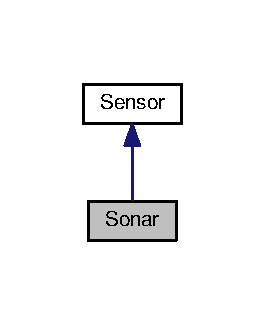
\includegraphics[width=127pt]{classSonar__inherit__graph}
\end{center}
\end{figure}


Collaboration diagram for Sonar\+:\nopagebreak
\begin{figure}[H]
\begin{center}
\leavevmode
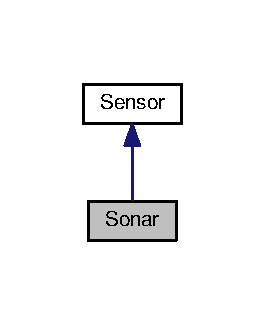
\includegraphics[width=127pt]{classSonar__coll__graph}
\end{center}
\end{figure}
\subsection*{Public Member Functions}
\begin{DoxyCompactItemize}
\item 
{\bfseries Sonar} (int sensor\+Handle)\hypertarget{classSonar_ae6edd4f329f9892a64c5f0cab808c7a2}{}\label{classSonar_ae6edd4f329f9892a64c5f0cab808c7a2}

\item 
int \hyperlink{classSonar_a6881d0c104c0fafad95ad1aea917b6f3}{get} (std\+::vector$<$ float $>$ \&detect\+Point, int \&detect\+Handle, std\+::vector$<$ float $>$ \&detect\+Surface)
\item 
int \hyperlink{classSonar_af77f9c5b9db42276b06b3b044c738284}{get} (std\+::vector$<$ float $>$ \&detect\+Point)
\item 
void \hyperlink{classSonar_ab32f714b0c5412e64ec60997467074bc}{update} (std\+::vector$<$ float $>$ \&f, int \&i, std\+::vector$<$ float $>$ \&ff)
\end{DoxyCompactItemize}
\subsection*{Additional Inherited Members}


\subsection{Member Function Documentation}
\index{Sonar@{Sonar}!get@{get}}
\index{get@{get}!Sonar@{Sonar}}
\subsubsection[{\texorpdfstring{get(std\+::vector$<$ float $>$ \&detect\+Point, int \&detect\+Handle, std\+::vector$<$ float $>$ \&detect\+Surface)}{get(std::vector< float > &detectPoint, int &detectHandle, std::vector< float > &detectSurface)}}]{\setlength{\rightskip}{0pt plus 5cm}int Sonar\+::get (
\begin{DoxyParamCaption}
\item[{std\+::vector$<$ float $>$ \&}]{detect\+Point, }
\item[{int \&}]{detect\+Handle, }
\item[{std\+::vector$<$ float $>$ \&}]{detect\+Surface}
\end{DoxyParamCaption}
)\hspace{0.3cm}{\ttfamily [virtual]}}\hypertarget{classSonar_a6881d0c104c0fafad95ad1aea917b6f3}{}\label{classSonar_a6881d0c104c0fafad95ad1aea917b6f3}
simply reads the sensor information with no additional call to handle the sensor in vrep 
\begin{DoxyParams}{Parameters}
{\em \&detect\+Point} & vector reference to store the coordinates of the closest point \\
\hline
{\em \&detect\+Handle} & integer reference to store the handle of the found object \\
\hline
{\em \&detect\+Surface} & vector reference to store the normal vector of the detected surface \\
\hline
\end{DoxyParams}


Implements \hyperlink{classSensor_a997a8679d48c4fa346e6ac43c1e6219a}{Sensor}.

\index{Sonar@{Sonar}!get@{get}}
\index{get@{get}!Sonar@{Sonar}}
\subsubsection[{\texorpdfstring{get(std\+::vector$<$ float $>$ \&detect\+Point)}{get(std::vector< float > &detectPoint)}}]{\setlength{\rightskip}{0pt plus 5cm}int Sonar\+::get (
\begin{DoxyParamCaption}
\item[{std\+::vector$<$ float $>$ \&}]{detect\+Point}
\end{DoxyParamCaption}
)\hspace{0.3cm}{\ttfamily [virtual]}}\hypertarget{classSonar_af77f9c5b9db42276b06b3b044c738284}{}\label{classSonar_af77f9c5b9db42276b06b3b044c738284}
same as the previous get, but all parameters except the coordinates of a detected point are omitted 

Implements \hyperlink{classSensor_a24f11619b11d5effc4066546629179ae}{Sensor}.

\index{Sonar@{Sonar}!update@{update}}
\index{update@{update}!Sonar@{Sonar}}
\subsubsection[{\texorpdfstring{update(std\+::vector$<$ float $>$ \&f, int \&i, std\+::vector$<$ float $>$ \&ff)}{update(std::vector< float > &f, int &i, std::vector< float > &ff)}}]{\setlength{\rightskip}{0pt plus 5cm}void Sonar\+::update (
\begin{DoxyParamCaption}
\item[{std\+::vector$<$ float $>$ \&}]{f, }
\item[{int \&}]{i, }
\item[{std\+::vector$<$ float $>$ \&}]{ff}
\end{DoxyParamCaption}
)\hspace{0.3cm}{\ttfamily [virtual]}}\hypertarget{classSonar_ab32f714b0c5412e64ec60997467074bc}{}\label{classSonar_ab32f714b0c5412e64ec60997467074bc}
calls for vrep to update the sensor information 
\begin{DoxyParams}{Parameters}
{\em \&detect\+Point} & vector reference to store the coordinates of the closest point \\
\hline
{\em \&detect\+Handle} & integer reference to store the handle of the found object \\
\hline
{\em \&detect\+Surface} & vector reference to store the normal vector of the detected surface \\
\hline
\end{DoxyParams}


Implements \hyperlink{classSensor_abb6c93c88529bc392d129443b3d352f3}{Sensor}.



The documentation for this class was generated from the following files\+:\begin{DoxyCompactItemize}
\item 
sonar.\+h\item 
sonar.\+cpp\end{DoxyCompactItemize}

\hypertarget{structSync}{}\section{Sync Struct Reference}
\label{structSync}\index{Sync@{Sync}}
\subsection*{Public Member Functions}
\begin{DoxyCompactItemize}
\item 
size\+\_\+t {\bfseries extend} ()\hypertarget{structSync_a12dd998a8af839e5e5663020f1607863}{}\label{structSync_a12dd998a8af839e5e5663020f1607863}

\item 
void {\bfseries set} (size\+\_\+t i)\hypertarget{structSync_a11ca0966d2a696487fd3eb2c5b85f393}{}\label{structSync_a11ca0966d2a696487fd3eb2c5b85f393}

\item 
{\bfseries operator bool} () const \hypertarget{structSync_a3a6cb3be79398ad788421bea42d90c7a}{}\label{structSync_a3a6cb3be79398ad788421bea42d90c7a}

\item 
void {\bfseries clear} ()\hypertarget{structSync_a41d73e5a06d373973cf50d439e132d11}{}\label{structSync_a41d73e5a06d373973cf50d439e132d11}

\end{DoxyCompactItemize}
\subsection*{Friends}
\begin{DoxyCompactItemize}
\item 
std\+::ostream \& {\bfseries operator$<$$<$} (std\+::ostream \&o, const \hyperlink{structSync}{Sync} s)\hypertarget{structSync_a1f4fd6c9f4d959c189137a370dc24d29}{}\label{structSync_a1f4fd6c9f4d959c189137a370dc24d29}

\end{DoxyCompactItemize}


The documentation for this struct was generated from the following file\+:\begin{DoxyCompactItemize}
\item 
thread\+Sync.\+cpp\end{DoxyCompactItemize}

\hypertarget{classVrepLog}{}\section{Vrep\+Log Class Reference}
\label{classVrepLog}\index{Vrep\+Log@{Vrep\+Log}}
\subsection*{Public Member Functions}
\begin{DoxyCompactItemize}
\item 
{\footnotesize template$<$typename T $>$ }\\\hyperlink{classLogLine}{Log\+Line} {\bfseries operator$<$$<$} (T \&t)\hypertarget{classVrepLog_a1a2744fc0ca891c3bf9767395791914b}{}\label{classVrepLog_a1a2744fc0ca891c3bf9767395791914b}

\end{DoxyCompactItemize}


The documentation for this class was generated from the following file\+:\begin{DoxyCompactItemize}
\item 
\hyperlink{finken_8h}{finken.\+h}\end{DoxyCompactItemize}

\hypertarget{classVREPPlugin}{}\section{V\+R\+E\+P\+Plugin Class Reference}
\label{classVREPPlugin}\index{V\+R\+E\+P\+Plugin@{V\+R\+E\+P\+Plugin}}


{\ttfamily \#include $<$vrepplugin.\+h$>$}



Inheritance diagram for V\+R\+E\+P\+Plugin\+:\nopagebreak
\begin{figure}[H]
\begin{center}
\leavevmode
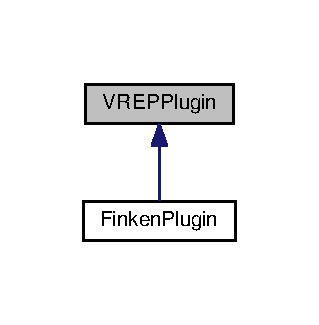
\includegraphics[width=153pt]{classVREPPlugin__inherit__graph}
\end{center}
\end{figure}
\subsection*{Public Member Functions}
\begin{DoxyCompactItemize}
\item 
\hyperlink{classVREPPlugin}{V\+R\+E\+P\+Plugin} \& {\bfseries operator=} (const \hyperlink{classVREPPlugin}{V\+R\+E\+P\+Plugin} \&)=delete\hypertarget{classVREPPlugin_aac9c374d0718ea48d6ec5baa8d8ab2b2}{}\label{classVREPPlugin_aac9c374d0718ea48d6ec5baa8d8ab2b2}

\item 
{\bfseries V\+R\+E\+P\+Plugin} (const \hyperlink{classVREPPlugin}{V\+R\+E\+P\+Plugin} \&)=delete\hypertarget{classVREPPlugin_accb66d8b1e8ded95475a15a3a42c9fbc}{}\label{classVREPPlugin_accb66d8b1e8ded95475a15a3a42c9fbc}

\item 
virtual unsigned char {\bfseries version} () const =0\hypertarget{classVREPPlugin_ae5e6764e97874aa134447122bbadbf2a}{}\label{classVREPPlugin_ae5e6764e97874aa134447122bbadbf2a}

\item 
virtual const std\+::string {\bfseries name} () const =0\hypertarget{classVREPPlugin_a345987cf0e2e8aa3af817cc0213e5c7a}{}\label{classVREPPlugin_a345987cf0e2e8aa3af817cc0213e5c7a}

\item 
virtual bool {\bfseries load} ()\hypertarget{classVREPPlugin_a4149b72b671ad72f63e9a75c58c0d628}{}\label{classVREPPlugin_a4149b72b671ad72f63e9a75c58c0d628}

\item 
virtual bool {\bfseries unload} ()\hypertarget{classVREPPlugin_a49aff8a71c1c9f2af6e32b918eba99ff}{}\label{classVREPPlugin_a49aff8a71c1c9f2af6e32b918eba99ff}

\item 
virtual void $\ast$ {\bfseries refresh\+Dialog} (int $\ast$auxiliary\+Data, void $\ast$custom\+Data, int $\ast$reply\+Data)\hypertarget{classVREPPlugin_aae582606dda4aff564d102358b9af579}{}\label{classVREPPlugin_aae582606dda4aff564d102358b9af579}

\item 
virtual void $\ast$ {\bfseries menu\+Item\+Selected} (int $\ast$auxiliary\+Data, void $\ast$custom\+Data, int $\ast$reply\+Data)\hypertarget{classVREPPlugin_a320dcb5ed4beaec82975be22b5c20e39}{}\label{classVREPPlugin_a320dcb5ed4beaec82975be22b5c20e39}

\item 
virtual void $\ast$ {\bfseries scene\+Content\+Change} (int $\ast$auxiliary\+Data, void $\ast$custom\+Data, int $\ast$reply\+Data)\hypertarget{classVREPPlugin_a7df55bb967c9f217c77add60bb0d3868}{}\label{classVREPPlugin_a7df55bb967c9f217c77add60bb0d3868}

\item 
virtual void $\ast$ {\bfseries instance\+Pass} (int $\ast$auxiliary\+Data, void $\ast$custom\+Data, int $\ast$reply\+Data)\hypertarget{classVREPPlugin_affe1c1f37ffa8e04ea93e9eda9399402}{}\label{classVREPPlugin_affe1c1f37ffa8e04ea93e9eda9399402}

\item 
virtual void $\ast$ {\bfseries instance\+Switch} (int $\ast$auxiliary\+Data, void $\ast$custom\+Data, int $\ast$reply\+Data)\hypertarget{classVREPPlugin_ae288b5fdec3fee292f23e61a021f4f5e}{}\label{classVREPPlugin_ae288b5fdec3fee292f23e61a021f4f5e}

\item 
virtual void $\ast$ {\bfseries main\+Script\+Call} (int $\ast$auxiliary\+Data, void $\ast$custom\+Data, int $\ast$reply\+Data)\hypertarget{classVREPPlugin_a5aa8491d41b377e75917ab1273674f9f}{}\label{classVREPPlugin_a5aa8491d41b377e75917ab1273674f9f}

\item 
virtual void $\ast$ {\bfseries sim\+Start} (int $\ast$auxiliary\+Data, void $\ast$custom\+Data, int $\ast$reply\+Data)\hypertarget{classVREPPlugin_a58c9675c38c6ca1a75047864d3e4253c}{}\label{classVREPPlugin_a58c9675c38c6ca1a75047864d3e4253c}

\item 
virtual void $\ast$ {\bfseries sim\+End} (int $\ast$auxiliary\+Data, void $\ast$custom\+Data, int $\ast$reply\+Data)\hypertarget{classVREPPlugin_a13ea56c8546d762468b21ebc141b4ca3}{}\label{classVREPPlugin_a13ea56c8546d762468b21ebc141b4ca3}

\item 
virtual void $\ast$ {\bfseries scene\+Load} (int $\ast$auxiliary\+Data, void $\ast$custom\+Data, int $\ast$reply\+Data)\hypertarget{classVREPPlugin_a77e10632cbc7ae0581a151daea83ab1f}{}\label{classVREPPlugin_a77e10632cbc7ae0581a151daea83ab1f}

\item 
virtual void $\ast$ {\bfseries open} (int $\ast$auxiliary\+Data, void $\ast$custom\+Data, int $\ast$reply\+Data)\hypertarget{classVREPPlugin_a40ededcae0889e8f8ecdf99d0f455179}{}\label{classVREPPlugin_a40ededcae0889e8f8ecdf99d0f455179}

\item 
virtual void $\ast$ {\bfseries action} (int $\ast$auxiliary\+Data, void $\ast$custom\+Data, int $\ast$reply\+Data)\hypertarget{classVREPPlugin_a048e1fbf7b4b5b7b96ea6ec132218e12}{}\label{classVREPPlugin_a048e1fbf7b4b5b7b96ea6ec132218e12}

\item 
virtual void $\ast$ {\bfseries close} (int $\ast$auxiliary\+Data, void $\ast$custom\+Data, int $\ast$reply\+Data)\hypertarget{classVREPPlugin_af9fc2e6b9adf1436fc06e2555eaa3c2b}{}\label{classVREPPlugin_af9fc2e6b9adf1436fc06e2555eaa3c2b}

\item 
virtual void $\ast$ {\bfseries save} (int $\ast$auxiliary\+Data, void $\ast$custom\+Data, int $\ast$reply\+Data)\hypertarget{classVREPPlugin_af6a19ea1a3fbe91a86df1e92e6f623a2}{}\label{classVREPPlugin_af6a19ea1a3fbe91a86df1e92e6f623a2}

\item 
virtual void $\ast$ {\bfseries render} (int $\ast$auxiliary\+Data, void $\ast$custom\+Data, int $\ast$reply\+Data)\hypertarget{classVREPPlugin_a3fce674766334a4ad6c63a179dff64ae}{}\label{classVREPPlugin_a3fce674766334a4ad6c63a179dff64ae}

\item 
virtual void $\ast$ {\bfseries broadcast} (int $\ast$auxiliary\+Data, void $\ast$custom\+Data, int $\ast$reply\+Data)\hypertarget{classVREPPlugin_aa04f0d2bb1b0d73a46a99e699e11830f}{}\label{classVREPPlugin_aa04f0d2bb1b0d73a46a99e699e11830f}

\item 
virtual void $\ast$ {\bfseries handle\+Other\+Message} (int message, int $\ast$auxiliary\+Data, void $\ast$custom\+Data, int $\ast$reply\+Data)\hypertarget{classVREPPlugin_af3a92d9202afe61bf4979d0e24bd5425}{}\label{classVREPPlugin_af3a92d9202afe61bf4979d0e24bd5425}

\end{DoxyCompactItemize}
\subsection*{Static Public Member Functions}
\begin{DoxyCompactItemize}
\item 
static \hyperlink{classVREPPlugin}{V\+R\+E\+P\+Plugin} \& {\bfseries get\+Instance} ()\hypertarget{classVREPPlugin_a6c54bebcd2d0c09e7a20dd72ae82ec71}{}\label{classVREPPlugin_a6c54bebcd2d0c09e7a20dd72ae82ec71}

\end{DoxyCompactItemize}


\subsection{Detailed Description}
Base vrepplugin class. Finkenplugin inherits from this class 

The documentation for this class was generated from the following files\+:\begin{DoxyCompactItemize}
\item 
vrepplugin.\+h\item 
vrepplugin.\+cpp\end{DoxyCompactItemize}

\chapter{File Documentation}
\hypertarget{finken_8h}{}\section{finken.\+h File Reference}
\label{finken_8h}\index{finken.\+h@{finken.\+h}}
{\ttfamily \#include \char`\"{}sensor.\+h\char`\"{}}\\*
{\ttfamily \#include $<$memory$>$}\\*
{\ttfamily \#include \char`\"{}sonar.\+h\char`\"{}}\\*
{\ttfamily \#include \char`\"{}heightsensor.\+h\char`\"{}}\\*
{\ttfamily \#include $<$rotor.\+h$>$}\\*
{\ttfamily \#include \char`\"{}positionsensor.\+h\char`\"{}}\\*
{\ttfamily \#include $<$v\+\_\+rep\+Lib.\+h$>$}\\*
{\ttfamily \#include $<$cstdlib$>$}\\*
{\ttfamily \#include $<$iostream$>$}\\*
{\ttfamily \#include $<$thread$>$}\\*
{\ttfamily \#include $<$utility$>$}\\*
{\ttfamily \#include $<$boost/asio.\+hpp$>$}\\*
{\ttfamily \#include $<$condition\+\_\+variable$>$}\\*
{\ttfamily \#include $<$chrono$>$}\\*
{\ttfamily \#include $<$Eigen/\+Dense$>$}\\*
{\ttfamily \#include $<$atomic$>$}\\*
{\ttfamily \#include $<$boost/filesystem.\+hpp$>$}\\*
{\ttfamily \#include $<$boost/filesystem/fstream.\+hpp$>$}\\*
Include dependency graph for finken.\+h\+:\nopagebreak
\begin{figure}[H]
\begin{center}
\leavevmode
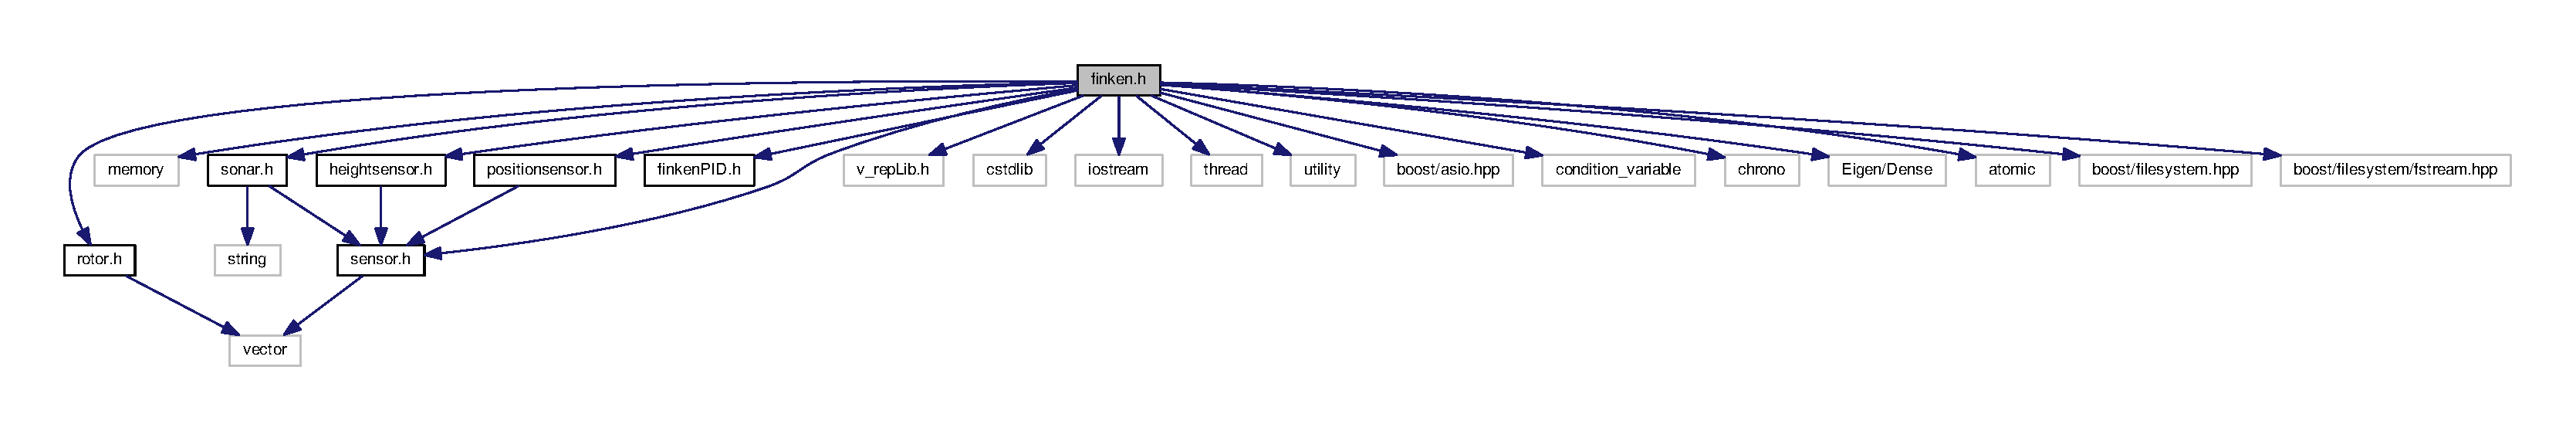
\includegraphics[width=350pt]{finken_8h__incl}
\end{center}
\end{figure}
\subsection*{Classes}
\begin{DoxyCompactItemize}
\item 
class \hyperlink{classLogLine}{Log\+Line}
\item 
class \hyperlink{classVrepLog}{Vrep\+Log}
\item 
class \hyperlink{classFinken}{Finken}
\end{DoxyCompactItemize}
\subsection*{Typedefs}
\begin{DoxyCompactItemize}
\item 
using {\bfseries Clock} = std\+::chrono\+::high\+\_\+resolution\+\_\+clock\hypertarget{finken_8h_accf829b29dcee7a09273bd9101f04e89}{}\label{finken_8h_accf829b29dcee7a09273bd9101f04e89}

\end{DoxyCompactItemize}
\subsection*{Functions}
\begin{DoxyCompactItemize}
\item 
void \hyperlink{finken_8h_a5810da3d23510cfe71d23902cddb8b51}{build\+Finken} (\hyperlink{classFinken}{Finken} \&finken, int handle)
\item 
double \hyperlink{finken_8h_a4e838d73ad5e098825ef4c227f6369b6}{thrust\+From\+Throttle} (double throttle)
\end{DoxyCompactItemize}
\subsection*{Variables}
\begin{DoxyCompactItemize}
\item 
std\+::atomic$<$ bool $>$ {\bfseries send\+Sync}\hypertarget{finken_8h_a97b68c87771b50f85a0c43bdb8410cbe}{}\label{finken_8h_a97b68c87771b50f85a0c43bdb8410cbe}

\item 
std\+::atomic$<$ bool $>$ {\bfseries read\+Sync}\hypertarget{finken_8h_a539cb20630c9a9a2583f643c0d6f36fa}{}\label{finken_8h_a539cb20630c9a9a2583f643c0d6f36fa}

\item 
\hyperlink{classVrepLog}{Vrep\+Log} {\bfseries vrep\+Log}\hypertarget{finken_8h_a89deba42952826c303251a9d4d45afda}{}\label{finken_8h_a89deba42952826c303251a9d4d45afda}

\item 
static std\+::vector$<$ std\+::unique\+\_\+ptr$<$ \hyperlink{classFinken}{Finken} $>$ $>$ \hyperlink{finken_8h_a16b7d4cd1197380860ab987e034385eb}{all\+Finken}
\end{DoxyCompactItemize}


\subsection{Function Documentation}
\index{finken.\+h@{finken.\+h}!build\+Finken@{build\+Finken}}
\index{build\+Finken@{build\+Finken}!finken.\+h@{finken.\+h}}
\subsubsection[{\texorpdfstring{build\+Finken(\+Finken \&finken, int handle)}{buildFinken(Finken &finken, int handle)}}]{\setlength{\rightskip}{0pt plus 5cm}void build\+Finken (
\begin{DoxyParamCaption}
\item[{{\bf Finken} \&}]{finken, }
\item[{int}]{handle}
\end{DoxyParamCaption}
)}\hypertarget{finken_8h_a5810da3d23510cfe71d23902cddb8b51}{}\label{finken_8h_a5810da3d23510cfe71d23902cddb8b51}
identifies a copter in the vrep scene using its handle and constructs it. Built finken are stored in \hyperlink{finken_8h_a16b7d4cd1197380860ab987e034385eb}{all\+Finken} \begin{DoxySeeAlso}{See also}
\hyperlink{classFinken_a4ac9d9b37fba41147a83a36286fbe91b}{Finken\+::add\+Rotor()} 

\hyperlink{classFinken_a2f2adb211e80a689f580b87730aeb9d1}{Finken\+::add\+Sensor()} 
\end{DoxySeeAlso}
\index{finken.\+h@{finken.\+h}!thrust\+From\+Throttle@{thrust\+From\+Throttle}}
\index{thrust\+From\+Throttle@{thrust\+From\+Throttle}!finken.\+h@{finken.\+h}}
\subsubsection[{\texorpdfstring{thrust\+From\+Throttle(double throttle)}{thrustFromThrottle(double throttle)}}]{\setlength{\rightskip}{0pt plus 5cm}double thrust\+From\+Throttle (
\begin{DoxyParamCaption}
\item[{double}]{throttle}
\end{DoxyParamCaption}
)}\hypertarget{finken_8h_a4e838d73ad5e098825ef4c227f6369b6}{}\label{finken_8h_a4e838d73ad5e098825ef4c227f6369b6}
Calculates thrust forces (Newton) from the rotor commands \begin{DoxySeeAlso}{See also}
\hyperlink{classFinken_aa4fe546d88b52ff92990bd67ced70567}{Finken\+::commands} 
\end{DoxySeeAlso}


\subsection{Variable Documentation}
\index{finken.\+h@{finken.\+h}!all\+Finken@{all\+Finken}}
\index{all\+Finken@{all\+Finken}!finken.\+h@{finken.\+h}}
\subsubsection[{\texorpdfstring{all\+Finken}{allFinken}}]{\setlength{\rightskip}{0pt plus 5cm}std\+::vector$<$std\+::unique\+\_\+ptr$<${\bf Finken}$>$ $>$ all\+Finken\hspace{0.3cm}{\ttfamily [static]}}\hypertarget{finken_8h_a16b7d4cd1197380860ab987e034385eb}{}\label{finken_8h_a16b7d4cd1197380860ab987e034385eb}
static vector containing all built finken 
%--- End generated contents ---

% Index
\backmatter
\newpage
\phantomsection
\clearemptydoublepage
\addcontentsline{toc}{chapter}{Index}
\printindex

\end{document}
